\section{A Conditional Uniqueness Theorem for the Dyck-Prefix Substrate}
\label{appendix:uniqueness}

This appendix isolates a minimal set of structural axioms under which the
Dyck-prefix substrate is not merely an example but is determined uniquely up to
isomorphism. The result is interpretation-neutral: it assumes no particular
computational semantics (evaluation order, combinators, rewriting), only a
ranked causal-growth structure with a one-sided admissibility boundary.

\subsection{Ranked growth posets}

\begin{definition}[Ranked growth poset]
\label{def:ranked-growth-poset}
A \emph{ranked growth poset} is a triple $(S,\preceq,\mathrm{rk})$ where $S$ is a
countable set, $\preceq$ is a partial order on $S$, and
$\mathrm{rk}:S\to\mathbb{N}$ is a rank function such that:
\begin{enumerate}[label=(\roman*)]
\item for every $t\in S$ the set $\{s\in S : s\preceq t\}$ is finite, and
\item $\mathrm{rk}$ is strictly order-increasing along cover relations.
\end{enumerate}
Write $s\prec t$ when $s\preceq t$ and $s\neq t$, and write
$s\lessdot t$ if $s\prec t$ and there is no $u$ with $s\prec u\prec t$
(i.e.\ $t$ \emph{covers} $s$).
\end{definition}

\begin{definition}[Two-move height structure]
\label{def:two-move-height}
Let $(S,\preceq,\mathrm{rk})$ be a ranked growth poset with a distinguished root
$s_{\emptyset}\in S$ satisfying $\mathrm{rk}(s_{\emptyset})=0$.
A \emph{two-move height structure} on $S$ consists of a function
$h:S\to\mathbb{Z}_{\ge 0}$ (height) with $h(s_{\emptyset})=0$ such that every
cover relation $s\lessdot t$ satisfies
\[
\mathrm{rk}(t)=\mathrm{rk}(s)+1
\qquad\text{and}\qquad
h(t)=h(s)\pm 1.
\]
We call a cover with $h(t)=h(s)+1$ an \emph{up-step} and a cover with
$h(t)=h(s)-1$ a \emph{down-step}.
\end{definition}

\subsection{Axioms for the Catalan core}

The uniqueness theorem below follows from four axioms capturing: (i) discrete
single-step growth, (ii) exactly two local move types (up/down), (iii) a
one-sided boundary in which down-steps are disabled at height $0$, and (iv) an
\emph{unfolded} (collision-free) history space.

\begin{definition}[Catalan core axioms]
\label{def:catalan-core-axioms}
A ranked growth poset $(S,\preceq,\mathrm{rk})$ with root $s_{\emptyset}$ and
two-move height structure $h$ satisfies the \emph{Catalan core axioms} if:
\begin{enumerate}[label=(A\arabic*)]
\item \textbf{(Ranked single-step growth)} For every cover $s\lessdot t$, one has
$\mathrm{rk}(t)=\mathrm{rk}(s)+1$ and $h(t)=h(s)\pm 1$.

\item \textbf{(Local determinism by move type)} For each $s\in S$, there exists
\emph{at most one} up-step successor $t_{\uparrow}$ with $s\lessdot t_{\uparrow}$
and $h(t_{\uparrow})=h(s)+1$, and \emph{at most one} down-step successor
$t_{\downarrow}$ with $s\lessdot t_{\downarrow}$ and $h(t_{\downarrow})=h(s)-1$.

\item \textbf{(One-sided boundary admissibility)} For each $s\in S$, an up-step
successor exists, while a down-step successor exists \emph{iff} $h(s)>0$.

\item \textbf{(No collisions / unique history)} Each $t\in S$ admits a unique
saturated chain (cover chain) from the root:
\[
s_{\emptyset}=s_0 \lessdot s_1 \lessdot \cdots \lessdot s_{\mathrm{rk}(t)}=t.
\]
\end{enumerate}
\end{definition}

\subsection{Dyck-prefix poset}

Let $\Sigma=\{+,-\}$. For a word $w=w_1\cdots w_n\in\Sigma^n$, define the
partial-sum height
\[
H_w(k)=\sum_{j=1}^k \xi(w_j),
\qquad
\text{where }\xi(+)=+1,\ \xi(-)=-1.
\]
Call $w$ \emph{admissible} if $H_w(k)\ge 0$ for all $k$.
Let $\mathcal{C}$ be the set of all admissible words (Dyck prefixes), partially
ordered by prefix: $u\preceq v$ iff $u$ is a prefix of $v$. Let $\ell(w)=n$ be
length and $H(w)=H_w(n)$ be final height.

\begin{definition}[Dyck-prefix poset]
\label{def:dyck-prefix-poset}
The \emph{Dyck-prefix poset} is $(\mathcal{C},\preceq,\ell)$ with root
$\varepsilon$ (the empty word).
\end{definition}

\subsection{Uniqueness theorem}

\begin{theorem}[Dyck-prefix uniqueness]
\label{thm:dyck-uniqueness}
Let $(S,\preceq,\mathrm{rk})$ be a ranked growth poset with root $s_{\emptyset}$
and a two-move height structure $h$. If $S$ satisfies the Catalan core axioms of
Definition~\ref{def:catalan-core-axioms}, then there exists a unique bijection
\[
\pi:S\to\mathcal{C}
\]
such that for every $s\in S$,
\[
\ell(\pi(s))=\mathrm{rk}(s),
\qquad
H(\pi(s))=h(s),
\]
and $\pi$ is an order isomorphism:
\[
s\preceq t \quad\Longleftrightarrow\quad \pi(s)\preceq \pi(t)
\quad\text{(prefix order).}
\]
In particular, $(S,\preceq,\mathrm{rk})$ is isomorphic to the Dyck-prefix poset.
\end{theorem}

\begin{proof}
By (A4), each $s\in S$ admits a unique cover chain
$s_{\emptyset}=s_0\lessdot\cdots\lessdot s_n=s$ where $n=\mathrm{rk}(s)$. Define
a word $\pi(s)\in\Sigma^n$ by setting
\[
\pi(s)_k=
\begin{cases}
+ & \text{if } h(s_k)=h(s_{k-1})+1,\\
- & \text{if } h(s_k)=h(s_{k-1})-1.
\end{cases}
\]
This is well-defined and has length $\ell(\pi(s))=n$. By construction, the
partial sums of $\pi(s)$ coincide with the height along the chain,
\[
H_{\pi(s)}(k)=h(s_k)\ge 0 \quad\text{for all }k,
\]
so $\pi(s)$ is admissible and $\pi(s)\in\mathcal{C}$. Moreover
$H(\pi(s))=H_{\pi(s)}(n)=h(s)$.

We now show that $\pi$ is bijective. Given any admissible word
$w=w_1\cdots w_n\in\mathcal{C}$, construct a chain in $S$ by starting at
$s_0=s_{\emptyset}$ and for each $k\ge 1$ taking the successor specified by
$w_k$:
\[
s_k=
\begin{cases}
\text{the (unique) up-step successor of } s_{k-1} & \text{if } w_k=+,\\
\text{the (unique) down-step successor of } s_{k-1} & \text{if } w_k=-.
\end{cases}
\]
Existence and uniqueness follow from (A2)--(A3); admissibility of $w$ ensures
that a down-step is only requested when the current height is positive. Let
$s:=s_n$ be the resulting node at rank $n$. Then $\pi(s)=w$, proving
surjectivity. Injectivity follows from (A4): distinct nodes have distinct
cover chains and hence distinct step sequences.

Finally, $\pi$ preserves order. If $s\preceq t$, then the unique chain to $t$
contains the chain to $s$ as an initial segment, so $\pi(s)$ is a prefix of
$\pi(t)$. Conversely, if $\pi(s)$ is a prefix of $\pi(t)$, then the constructed
chain for $\pi(t)$ passes through the constructed chain for $\pi(s)$, giving
$s\preceq t$. Uniqueness of $\pi$ is immediate from (A4), since $\pi(s)$ is
forced by the unique cover chain to~$s$.
\end{proof}

\subsection{Catalan enumeration at completion}

To recover the usual Catalan counting, impose a completion boundary condition:
completion occurs when the height returns to zero at even rank.

\begin{definition}[Completed histories]
\label{def:completed-histories}
For $n\in\mathbb{N}$, define the set of \emph{completed histories} at rank $2n$ by
\[
S^{\mathrm{comp}}_{2n} := \{s\in S : \mathrm{rk}(s)=2n \text{ and } h(s)=0\}.
\]
\end{definition}

\begin{corollary}[Catalan counting]
\label{cor:catalan-counting}
Under the hypotheses of Theorem~\ref{thm:dyck-uniqueness}, the number of
completed histories satisfies
\[
\#\bigl(S^{\mathrm{comp}}_{2n}\bigr)=C_n
=\frac{1}{n+1}\binom{2n}{n},
\]
the $n$th Catalan number.
\end{corollary}

\begin{proof}
By Theorem~\ref{thm:dyck-uniqueness}, $S^{\mathrm{comp}}_{2n}$ is in bijection
with admissible words of length $2n$ with final height $0$, i.e.\ Dyck words of
semilength $n$. These are counted by the Catalan number $C_n$.
\end{proof}

\subsection{Quotients and structural sharing}

The ``no collisions'' axiom (A4) asserts that $S$ is an \emph{unfolded} history
space: each node encodes a distinct growth history. This does not preclude gauge
equivalences or multi-way computation graphs; rather, those arise by quotienting
$S$ by an equivalence relation.

\begin{remark}[Quotients and gauge identification]
\label{rem:gauge-quotient}
Let $\sim$ be an equivalence relation on $S$ representing gauge or rewrite
identifications. The quotient set $S/{\sim}$ may exhibit merges (a DAG-like
state graph), even if $S$ is collision-free. Theorem~\ref{thm:dyck-uniqueness}
characterizes the unfolded core; quotient structure is encoded by the choice of
$\sim$ and acts as an identification of histories rather than a primitive
feature of the substrate.
\end{remark}

\begin{remark}[Structural sharing vs.\ semantic collisions]
\label{rem:sharing}
Axiom (A4) concerns semantic identity in $S$ (distinct histories are distinct
nodes). It is compatible with immutability and structural sharing in
implementations (e.g.\ hash-consing), which may share representation of common
substructures without identifying distinct history nodes.
\end{remark}

\subsection{Scope of the result}

Theorem~\ref{thm:dyck-uniqueness} establishes a core uniqueness statement:
given two local move types changing an integer height by $\pm 1$, a one-sided
boundary disabling down-steps at height $0$, and an unfolded history space, the
substrate is forced to be Dyck-prefix order. This statement is independent of
additional semantic layers (program interpretations, rewriting dynamics, or
amplitude assignments), which can be imposed on top of the substrate without
affecting the isomorphism.

\section{Unfoldings and Covers of Growth Posets}
\label{appendix:unfoldings}

Many natural representations of computation or gauge-identified state spaces
exhibit merges: distinct growth histories may lead to the same state, producing
a DAG-like multi-way graph rather than a tree. The core uniqueness theorem in
Appendix~\ref{appendix:uniqueness} characterizes the \emph{unfolded} history
space. This appendix makes that relationship explicit by defining a canonical
unfolding (history cover) for a ranked growth poset and showing that the Catalan
uniqueness statement applies upstairs even when merges exist downstairs.

\subsection{Growth graphs}

\begin{definition}[Rooted ranked growth poset]
\label{def:rooted-ranked-growth-poset}
A \emph{rooted ranked growth poset} is a ranked growth poset
$(S,\preceq,\mathrm{rk})$ (Definition~\ref{def:ranked-growth-poset}) equipped
with a distinguished root $s_{\emptyset}\in S$ such that for every $s\in S$ one
has $s_{\emptyset}\preceq s$ (i.e.\ every node is reachable from the root).
\end{definition}

\begin{definition}[Directed growth graph]
\label{def:directed-growth-graph}
Let $(S,\preceq,\mathrm{rk})$ be a rooted ranked growth poset.
Its \emph{directed growth graph} is the rooted directed graph
$G(S)=(V,E,s_{\emptyset})$ where $V=S$ and $(s,t)\in E$ iff $s\lessdot t$
(i.e.\ $t$ covers $s$). We regard each edge as a single-step growth move.
\end{definition}

\begin{definition}[Move type induced by height]
\label{def:move-type}
If $(S,\preceq,\mathrm{rk})$ carries a two-move height structure $h$
(Definition~\ref{def:two-move-height}), then each directed edge $s\to t$ in
$G(S)$ has a \emph{move type}
\[
\mathrm{type}(s\to t)\in\{+,-\}
\quad\text{defined by}\quad
\mathrm{type}(s\to t)=
\begin{cases}
+ & \text{if } h(t)=h(s)+1,\\
- & \text{if } h(t)=h(s)-1.
\end{cases}
\]
\end{definition}

\subsection{Rooted covers (local isomorphism in one step)}

To model ``the same local growth rule everywhere'' we use a minimal notion of
cover: a map that is locally bijective on outgoing edges from each node. This
avoids introducing general poset coverings and suffices for the unfolding
argument below.

\begin{definition}[Rooted directed cover]
\label{def:rooted-directed-cover}
Let $G=(V,E,r)$ and $\widetilde{G}=(\widetilde{V},\widetilde{E},\widetilde{r})$
be rooted directed graphs. A function $\varphi:\widetilde{V}\to V$ is a
\emph{rooted directed cover} if:
\begin{enumerate}[label=(\roman*)]
\item $\varphi(\widetilde{r})=r$;
\item for every $\widetilde{v}\in\widetilde{V}$, the map
\[
\varphi_*:\mathrm{Out}(\widetilde{v})\to \mathrm{Out}(\varphi(\widetilde{v})),
\qquad
(\widetilde{v}\to \widetilde{w})\mapsto (\varphi(\widetilde{v})\to \varphi(\widetilde{w}))
\]
is a bijection, where $\mathrm{Out}(x)=\{x\to y\in E\}$ denotes the set of
outgoing edges from $x$.
\end{enumerate}
If edges carry move types $\{+,-\}$, we additionally require that $\varphi_*$
preserves move type (i.e.\ the bijection matches $+$-edges to $+$-edges and
$-$-edges to $-$-edges).
\end{definition}

\subsection{The canonical unfolding (history cover)}

\begin{definition}[Unfolding as rooted path space]
\label{def:unfolding}
Let $(S,\preceq,\mathrm{rk})$ be a rooted ranked growth poset and let $G(S)$ be
its directed growth graph.
Define the \emph{unfolding} $\widetilde{S}$ to be the set of all finite directed
paths in $G(S)$ starting at the root:
\[
\widetilde{S}
:=\bigl\{
(s_0\to s_1\to\cdots\to s_n)\ :\ s_0=s_{\emptyset},\ (s_{k-1},s_k)\in E
\bigr\}.
\]
Write $\widetilde{s}=(s_0\to\cdots\to s_n)$ and define:
\begin{enumerate}[label=(\roman*)]
\item the \emph{endpoint} map $\varphi:\widetilde{S}\to S$ by
$\varphi(\widetilde{s})=s_n$;
\item the \emph{rank} $\widetilde{\mathrm{rk}}(\widetilde{s})=n$ (path length);
\item the \emph{prefix order} on $\widetilde{S}$:
$\widetilde{u}\preceq \widetilde{v}$ iff $\widetilde{u}$ is an initial segment
(prefix) of $\widetilde{v}$.
\end{enumerate}
If $S$ has a height function $h$, define the lifted height
$\widetilde{h}(\widetilde{s}) := h(\varphi(\widetilde{s}))$.
\end{definition}

\begin{lemma}[The unfolding is collision-free]
\label{lem:unfolding-collision-free}
Every element $\widetilde{s}\in\widetilde{S}$ has a unique predecessor chain
from the root in the prefix order, i.e.\ $\widetilde{S}$ satisfies the ``no
collisions / unique history'' property (A4) of
Definition~\ref{def:catalan-core-axioms}.
\end{lemma}

\begin{proof}
By construction, each $\widetilde{s}$ is itself a rooted path
$(s_0\to\cdots\to s_n)$. Its strict prefixes are exactly the initial segments
$(s_0\to\cdots\to s_k)$ for $0\le k<n$, and these form the unique saturated
chain from the root to $\widetilde{s}$ under prefix inclusion.
\end{proof}

\begin{lemma}[The endpoint map is a rooted directed cover]
\label{lem:endpoint-cover}
Let $G(\widetilde{S})$ be the directed growth graph of the unfolding, whose
edges append one growth step:
\[
(s_0\to\cdots\to s_n)\ \to\ (s_0\to\cdots\to s_n\to s_{n+1})
\quad\text{whenever } s_n\to s_{n+1}\text{ is an edge in }G(S).
\]
Then the endpoint map $\varphi:\widetilde{S}\to S$ from
Definition~\ref{def:unfolding} is a rooted directed cover in the sense of
Definition~\ref{def:rooted-directed-cover}. If $S$ carries a two-move height
structure, then $\varphi$ preserves move type.
\end{lemma}

\begin{proof}
Clearly $\varphi$ maps the length-$0$ path $(s_{\emptyset})$ to $s_{\emptyset}$.
Fix a path $\widetilde{s}=(s_0\to\cdots\to s_n)$. Outgoing edges from
$\widetilde{s}$ in $G(\widetilde{S})$ are in bijection with outgoing edges from
$s_n$ in $G(S)$ by appending the corresponding last step $s_n\to s_{n+1}$. Under
$\varphi$, each appended edge maps to exactly that edge $s_n\to s_{n+1}$, giving
a bijection on outgoing edges. If move types are present, appending an up-step
or down-step in $\widetilde{S}$ maps to an up-step or down-step in $S$ by
Definition~\ref{def:move-type}, so type is preserved.
\end{proof}

\subsection{Dyck-prefix structure upstairs}

\begin{proposition}[Lift of the Catalan core axioms]
\label{prop:lift-axioms}
Suppose $(S,\preceq,\mathrm{rk})$ is a rooted ranked growth poset with a two-move
height structure $h$ satisfying axioms (A1)--(A3) of
Definition~\ref{def:catalan-core-axioms} (ranked single-step growth, local
determinism by move type, and one-sided boundary admissibility), but not
necessarily (A4). Then the unfolding $(\widetilde{S},\preceq,\widetilde{\mathrm{rk}})$
with lifted height $\widetilde{h}$ satisfies (A1)--(A4).
\end{proposition}

\begin{proof}
Axiom (A4) holds by Lemma~\ref{lem:unfolding-collision-free}. For (A1)--(A3),
each cover in $\widetilde{S}$ appends exactly one edge of $G(S)$, so ranks
increase by one and height changes by $\pm 1$ exactly as in $S$. Moreover, by
local determinism in $S$, from any endpoint there is at most one $+$-successor
and at most one $-$-successor; by Lemma~\ref{lem:endpoint-cover} the same holds
in the unfolding at every path. Finally, one-sided boundary admissibility is
preserved: a $-$-extension exists in $\widetilde{S}$ precisely when the endpoint
height is positive.
\end{proof}

\begin{theorem}[Dyck-prefix characterization of the unfolding]
\label{thm:dyck-unfolding}
Under the hypotheses of Proposition~\ref{prop:lift-axioms}, the unfolding
$\widetilde{S}$ is (canonically) order-isomorphic to the Dyck-prefix poset
(Definition~\ref{def:dyck-prefix-poset}). In particular, completed unfolded
histories are counted by Catalan numbers as in Corollary~\ref{cor:catalan-counting}.
\end{theorem}

\begin{proof}
By Proposition~\ref{prop:lift-axioms}, $\widetilde{S}$ satisfies the full Catalan
core axioms (A1)--(A4). The conclusion follows by applying
Theorem~\ref{thm:dyck-uniqueness} to $\widetilde{S}$.
\end{proof}

\begin{remark}[Canonical quotient and ``collisions'']
\label{rem:canonical-quotient}
The unfolding comes with a canonical surjection $\varphi:\widetilde{S}\to S$
(the endpoint map). Collisions/merges in $S$ correspond exactly to
identifications of distinct unfolded histories:
\[
\widetilde{u}\sim_{\varphi}\widetilde{v}
\quad\Longleftrightarrow\quad
\varphi(\widetilde{u})=\varphi(\widetilde{v}).
\]
Thus, as a set of states reachable from the root, $S$ is naturally identified
with the quotient $\widetilde{S}\big/\!\sim_{\varphi}$.
For the distinction between semantic identification and structural sharing in
implementations, see Remark~\ref{rem:sharing}.
\end{remark}

\subsection{A Reduction-Theoretic ``Full Uniqueness'' Statement}
\label{subsec:full-uniqueness}

The core uniqueness theorem (Theorem~\ref{thm:dyck-uniqueness}) shows that a
collision-free two-move growth system with a one-sided boundary is forced to be
Dyck-prefix order. This subsection records a complementary reduction statement:
if a canonical notion of \emph{intrinsic state} (defined by future-cone
isomorphism) is already a minimal one-counter system, and if the projection to
intrinsic state is locally bijective on labeled moves, then the Catalan core is
forced as the unfolded normal form.

\subsubsection{Future cones and intrinsic-state equivalence}

\begin{definition}[Future cone as a rooted directed graph]
\label{def:future-cone}
Let $(S,\preceq,\mathrm{rk})$ be a rooted ranked growth poset with directed
growth graph $G(S)=(S,E,s_{\emptyset})$ (Definition~\ref{def:directed-growth-graph}).
For $s\in S$, define the \emph{future cone} at $s$ to be the rooted directed
subgraph
\[
\mathrm{Cone}(s)\ :=\ \bigl(S_s,E_s,s\bigr),
\]
where $S_s=\{t\in S:\ s\preceq t\}$ and $E_s=\{(u,v)\in E:\ u,v\in S_s\}$. If
edges in $G(S)$ are labeled by a finite move alphabet (in particular $\{+,-\}$),
we regard $\mathrm{Cone}(s)$ as an edge-labeled rooted directed graph.
\end{definition}

\begin{definition}[Cone isomorphism and intrinsic-state equivalence]
\label{def:cone-iso}
Assume edges are labeled by move type in $\{+,-\}$. For $s,t\in S$, write
$s\equiv t$ if there exists a rooted directed graph isomorphism
\[
\psi:\mathrm{Cone}(s)\ \cong\ \mathrm{Cone}(t)
\]
sending root to root and preserving move labels. This defines an equivalence
relation $\equiv$ on $S$, called \emph{intrinsic-state equivalence}. Let
$M:=S/{\equiv}$ be the set of equivalence classes, with root
$m(s_{\emptyset})\in M$, and write
\[
m:S\to M,\qquad m(s)=[s]_{\equiv}
\]
for the canonical projection.
\end{definition}

\begin{remark}[Relocatable futures]
\label{rem:relocatable}
The equivalence relation $\equiv$ captures a precise form of relocatability:
states are indistinguishable if and only if their reachable futures are
isomorphic as rooted labeled growth graphs. The quotient $M=S/{\equiv}$ is a
canonical ``coarsest'' state descriptor that preserves the full future growth
structure.
\end{remark}

\subsubsection{Intrinsic dynamics and the cover hypothesis}

\begin{definition}[Intrinsic transition graph]
\label{def:intrinsic-transition}
Let $G(S)$ be labeled by $\{+,-\}$. Define a rooted labeled directed graph
$G(M)$ on $M$ by declaring a labeled edge $x\to_{\pm} y$ to exist if there are
$s,t\in S$ such that $s\lessdot t$ is a $\pm$-labeled edge of $G(S)$ and
$m(s)=x$, $m(t)=y$.
\end{definition}

\begin{definition}[One-counter intrinsic dynamics]
\label{def:one-counter-dynamics}
We say $(S,\preceq,\mathrm{rk})$ has \emph{one-counter intrinsic dynamics} if
there exists a bijection
\[
\iota: M \ \to\ \mathbb{Z}_{\ge 0}
\]
with $\iota(m(s_{\emptyset}))=0$ such that, for every intrinsic state $x\in M$
with $\iota(x)=k$:
\begin{enumerate}[label=(\roman*)]
\item (\textbf{Two primitive moves}) there exists exactly one $+$-successor
$y_{+}$ of $x$ in $G(M)$ with $\iota(y_{+})=k+1$;
\item (\textbf{One-sided boundary}) there exists a $-$-successor $y_{-}$ of $x$
in $G(M)$ iff $k>0$, and in that case $\iota(y_{-})=k-1$;
\item (\textbf{No other intrinsic moves}) $x$ has no other outgoing edges in
$G(M)$ besides $x\to_{+}y_{+}$ and (when $k>0$) $x\to_{-}y_{-}$.
\end{enumerate}
Equivalently, $G(M)$ is isomorphic (as a rooted labeled graph) to the standard
one-counter graph on $\mathbb{Z}_{\ge 0}$ with edges $k\to_{+} k+1$ for all $k$
and edges $k\to_{-} k-1$ for $k>0$.
\end{definition}

\begin{remark}[Minimality content]
\label{rem:minimality-content}
Definition~\ref{def:one-counter-dynamics} should be read as a minimality
hypothesis: the intrinsic descriptor $M=S/{\equiv}$ is already a single
nonnegative integer, and it admits exactly two primitive move types with a
one-sided boundary at~$0$.
\end{remark}

\begin{definition}[Cover-consistency of the intrinsic projection]
\label{def:intrinsic-cover}
Assume edges are labeled by $\{+,-\}$. We say the intrinsic projection
$m:S\to M$ is \emph{cover-consistent} if it is a rooted directed cover
(Definition~\ref{def:rooted-directed-cover}) from the labeled growth graph
$G(S)$ to the intrinsic graph $G(M)$ (Definition~\ref{def:intrinsic-transition}),
i.e.\ for every $s\in S$ the induced map on outgoing edges
$\mathrm{Out}(s)\to\mathrm{Out}(m(s))$ is a label-preserving bijection.
\end{definition}

\begin{remark}
Under the one-counter identification $\iota:M\to\mathbb{Z}_{\ge 0}$ of
Definition~\ref{def:one-counter-dynamics}, cover-consistency of $m$ is
equivalent to requiring that the composite $h:=\iota\circ m:S\to\mathbb{Z}_{\ge 0}$
is a rooted directed cover from $G(S)$ to the standard one-counter graph on
$\mathbb{Z}_{\ge 0}$.
\end{remark}

\subsubsection{Reduction to the Dyck-prefix normal form}

\begin{theorem}[Reduction to a Dyck-prefix cover]
\label{thm:full-uniqueness-reduction}
Let $(S,\preceq,\mathrm{rk})$ be a rooted ranked growth poset whose directed
growth graph $G(S)$ is labeled by move type in $\{+,-\}$. Assume:
\begin{enumerate}[label=(H\arabic*)]
\item \textbf{(Intrinsic-state quotient)} intrinsic-state equivalence $\equiv$ is
defined by label-preserving cone isomorphism as in Definition~\ref{def:cone-iso},
with quotient $m:S\to M$;
\item \textbf{(One-counter intrinsic dynamics)} $S$ satisfies
Definition~\ref{def:one-counter-dynamics};
\item \textbf{(Cover consistency)} the intrinsic projection $m$ is a rooted
directed cover as in Definition~\ref{def:intrinsic-cover};
\item \textbf{(Tiered single-step growth)} for every cover $s\lessdot t$,
$\mathrm{rk}(t)=\mathrm{rk}(s)+1$.
\end{enumerate}
Let $\widetilde{S}$ be the unfolding (history cover) of $S$ (Definition~\ref{def:unfolding})
with endpoint map $\varphi:\widetilde{S}\to S$. Then $\widetilde{S}$ is
(canonically) order-isomorphic to the Dyck-prefix poset (Definition~\ref{def:dyck-prefix-poset}),
and hence $S$ is a quotient (folding) of a Dyck-prefix cover via~$\varphi$
(Remark~\ref{rem:canonical-quotient}).
\end{theorem}

\begin{proof}
Define a height function on $S$ by composing the intrinsic-state projection with
the one-counter identification,
\[
h(s)\;:=\;\iota(m(s))\in\mathbb{Z}_{\ge 0}.
\]
By cover consistency (Definition~\ref{def:intrinsic-cover}) and one-counter
intrinsic dynamics (Definition~\ref{def:one-counter-dynamics}), each $s\in S$
has exactly one outgoing $+$-edge, and it has an outgoing $-$-edge iff $h(s)>0$.
Moreover, because $m$ is label-preserving and $\iota$ identifies $G(M)$ with the
standard one-counter graph, along any cover edge $s\lessdot t$ one has
$h(t)=h(s)+1$ for a $+$-edge and $h(t)=h(s)-1$ for a $-$-edge. Together with the
tier assumption $\mathrm{rk}(t)=\mathrm{rk}(s)+1$, this shows that $S$ admits a
two-move height structure satisfying axioms (A1)--(A3) of
Definition~\ref{def:catalan-core-axioms}.

Applying Theorem~\ref{thm:dyck-unfolding} now yields that the unfolding
$\widetilde{S}$ is Dyck-prefix order-isomorphic. The quotient statement for $S$
is then exactly Remark~\ref{rem:canonical-quotient}.
\end{proof}

\begin{remark}[What is and is not proved]
\label{rem:what-is-not-proved}
Theorem~\ref{thm:full-uniqueness-reduction} is a ``full uniqueness'' statement
in the reduction sense: once relocatable futures are formalized via cone
isomorphism and the intrinsic state space is assumed to be a one-counter with
two primitive moves, together with the cover-consistency hypothesis (no hidden
multiplicity in the projection $m$), the Catalan substrate is forced as the
unfolded normal form. What is not claimed is that all reasonable substrates
satisfy these minimality hypotheses; establishing that requires separate
domain-specific arguments.
\end{remark}

\subsection{Interpretive takeaway}

Theorems~\ref{thm:dyck-uniqueness} and~\ref{thm:dyck-unfolding} together support
the following robust core statement: whenever a ranked two-move growth system
with a one-sided boundary is present, the unfolded history space is forced to be
Dyck-prefix order, and any merged multi-way representation is a quotient of that
Catalan cover.

\section{Additional Technical Notes}
\label{appendix:technical-notes}

\noindent
This appendix collects optional bookkeeping and auxiliary constructions. It is
separate from the main formal development and may be skipped on first reading.

\subsection{Entropy of coarse-graining and information rate}

Fix a tier $n$ and an observable (deterministic coarse-graining)
$f:\mathcal D_n\to\mathcal X$. For $x\in\mathcal X$ write
\[
N(x)\;:=\;\#\{w\in \mathcal D_n: f(w)=x\},
\]
so that $f^{-1}(x)$ is the equivalence class of histories identified as the
same outcome.
If $f$ is prefix-local in the sense of Remark~\mainref{rem:local-observables}, then
the multiplicities $N(x)$ admit transfer recursions on the induced state space.

\paragraph{Multiplicity entropy.}
Define the (microcanonical) entropy of the full ensemble at tier $n$ by
\[
S_n \;:=\; \log \#(\mathcal D_n),
\]
and the conditional entropy of an outcome $x$ by
\[
S(x) \;:=\; \log N(x).
\]
The information eliminated by selecting outcome $x$ is the entropy drop
\[
\Delta S(x)\;:=\; S_n - S(x)
\;=\; \log\!\Big(\frac{\#(\mathcal D_n)}{N(x)}\Big).
\]
(Any logarithm base may be used; base $2$ yields units of bits.)

\begin{remark}[Retrospective vs.\ prospective counts]
The multiplicity entropy $S(x)=\log N(x)$ measures how many fine-grained
histories are identified as the same outcome at tier $n$. A complementary
forward-looking quantity is the number of admissible continuations of a
realized prefix into higher tiers (the size of its local cone; see
Section~\mainref{sec:multiplecones}), which may be studied by counting completions
as a function of current height (Lemma~\mainref{lem:ballot-completions}).
\end{remark}

\paragraph{Completion multiplicity and future-cone entropy.}
Fix a Dyck prefix $u$ of length $k$ and height $h$. For a target tier $n$ with
$2n\ge k$, define the completion multiplicity
\[
M_n(u)\;:=\;\#\{w\in \mathcal D_n : u\preceq w\},
\]
	the number of completed histories at tier $n$ consistent with the partial
	history $u$. This is the finite-tier size of the local cone rooted at $u$.
	It depends only on the remaining step budget $s:=2n-k$ and the current height
	$h$, and admits the explicit ballot-number formula of
	Lemma~\mainref{lem:ballot-completions}. The associated future-cone entropy is
\[
	S^{\mathrm{cone}}_n(u)\;:=\;\log M_n(u).
\]

\paragraph{Information rate as rate of possibility reduction.}
Let $m$ denote the number of selection events (local contractions) along a
history, and let computational proper time be $\tau=\tau_0 m$ for a fixed scale
$\tau_0>0$. We define the information rate associated with outcome $x$ to be the
information loss per unit computational proper time,
\[
R(x)\;:=\;\frac{\Delta S(x)}{\tau}.
\]
In the simplest case of a single event ($m=1$), this reduces to
$R(x)=\Delta S(x)/\tau_0$.
One may also adopt a coarser tier-wise selection model in which $m$ is
identified with the tier index $n$ (one selection per tier boundary), but we
keep these notions separate in general.

\paragraph{Gauge-invariant counting.}
When histories admit a redundancy under commuting spacelike-separated updates,
one may quotient the fine-grained history set at tier $n$ by the induced gauge
equivalence relation $\sim_g$ of Definition~\mainref{def:gauge-equivalence}. When
$\mathcal D_n$ is taken to parametrize such fine-grained histories at tier $n$,
define $\bar{\mathcal D}_n:=\mathcal D_n/\!\sim_g$. If $f$ is gauge-invariant
(constant on $\sim_g$-orbits), define
\[
\bar N(x):=\#\{[w]\in \bar{\mathcal D}_n : f(w)=x\},
\qquad
\bar{\Delta S}(x):=\log\!\Big(\frac{\#(\bar{\mathcal D}_n)}{\bar N(x)}\Big),
\]
and use $\bar{\Delta S}$ in place of $\Delta S$. This removes overcounting due
solely to reordering of independent collapses.

\subsection{Size bookkeeping for subtree-selection collapses}
\label{subsec:collapse-size}

In addition to ensemble-level multiplicities, some collapse rules admit a simple
size bookkeeping at the level of individual trees. Let $T$ be a finite full
binary tree. Define its \emph{internal size} $U(T)$ (number of internal nodes)
recursively by
\[
U(\texttt{()}) := 0,\qquad
U(\bullet(L,R)) := 1 + U(L) + U(R),
\]
where $\texttt{()}$ denotes a leaf and $\bullet(L,R)$ denotes a binary pair.

\begin{lemma}[Size drop under subtree selection]
\label{lem:subtree-selection-drop}
Consider the local collapse that replaces a pair $\bullet(L,R)$ by one of its
children:
\[
\bullet(L,R)\;\rightsquigarrow\; L
\qquad\text{or}\qquad
\bullet(L,R)\;\rightsquigarrow\; R.
\]
Then the size drop is
\[
U(\bullet(L,R)) - U(L) = 1 + U(R),
\qquad
U(\bullet(L,R)) - U(R) = 1 + U(L).
\]
In particular, if the collapse rule keeps the larger child in $U$ (i.e.\ keeps
$\arg\max\{U(L),U(R)\}$), then the drop is $1+\min\{U(L),U(R)\}$.
\end{lemma}

\begin{proof}
Immediate from the defining recursion $U(\bullet(L,R))=1+U(L)+U(R)$.
\end{proof}

% Optional operator/field frameworks (operators on tiers/trees, Laplacians, etc.).
% Supplemental material extracted from `docs/catalan-light-cone.tex`.
% This block was removed from the compiled arXiv PDF to keep the main v1 lean.
% Intended use: `\% Supplemental material extracted from `docs/catalan-light-cone.tex`.
% This block was removed from the compiled arXiv PDF to keep the main v1 lean.
% Intended use: `\% Supplemental material extracted from `docs/catalan-light-cone.tex`.
% This block was removed from the compiled arXiv PDF to keep the main v1 lean.
% Intended use: `\\input{supplemental-operators.tex}` at the former location in
% Appendix "Additional Technical Notes".

\subsection{Fields on words, prefixes, and nodes (optional)}
\label{subsec:fields}

We use the word ``field'' as shorthand for a complex-valued function on one of
the Catalan objects already in play. Several closely related state spaces are
useful in different contexts.

\paragraph{Fields on completed histories (fixed tier).}
Fix $n$ and consider a function $\Phi_n:\mathcal D_n\to\mathbb{C}$ assigning an
amplitude (or observable value) to each completed history $w\in\mathcal D_n$.
The associated Hilbert space is $\ell^2(\mathcal D_n)$ with inner product
\[
\langle \psi,\phi\rangle := \sum_{w\in\mathcal D_n} \overline{\psi(w)}\,\phi(w).
\]

\paragraph{Fields on prefixes (the full cone).}
Let $\mathcal{C}$ denote the set of Dyck prefixes (admissible partial histories).
A prefix field is a function $\Phi:\mathcal{C}\to\mathbb{C}$, which may be
restricted to a fixed length slice
$\mathcal{C}^{(k)}:=\{p\in\mathcal{C}: |p|=k\}$ when needed.

\paragraph{Fields on nodes of a fixed tree.}
Given $w\in\mathcal D_n$, let $T(w)$ be its associated full binary tree. A
node field is a function $\phi_w:\mathrm{Int}(T(w))\to\mathbb{C}$ on the internal
nodes of that tree.

\begin{remark}
These notions live on different objects (tiers, the prefix poset, or a single
tree) and are independent of any within-tier ordering convention on
$\mathcal D_n$.
\end{remark}

\subsection{Subtree indicators as a multiscale spanning family (optional)}
\label{subsec:subtree-indicators}

Let $T$ be a finite rooted tree and write $\mathrm{Int}(T)$ for its internal
nodes. Each $v\in\mathrm{Int}(T)$ determines a rooted subtree $T_v$, and hence a
subset $\mathrm{Int}(T_v)\subseteq \mathrm{Int}(T)$. Define the subtree indicator
\[
\chi_v:\mathrm{Int}(T)\to\{0,1\},
\qquad
\chi_v(u):=\mathbf{1}\{u\in \mathrm{Int}(T_v)\}.
\]

\begin{lemma}[Subtree indicators form a basis]
\label{lem:subtree-indicator-basis}
The family $\{\chi_v: v\in \mathrm{Int}(T)\}$ is a basis of the vector space of
complex-valued functions on $\mathrm{Int}(T)$.
\end{lemma}

\begin{proof}
Order the internal nodes by nonincreasing depth (deepest first), and let $M$ be
the square matrix with entries $M_{uv}:=\chi_v(u)$. Then $M_{vv}=1$ for all $v$,
while $M_{uv}=0$ whenever $u$ precedes $v$ in this order (a node cannot be a
descendant of a deeper node). Thus $M$ is triangular with ones on the diagonal,
hence invertible. Therefore the indicators are linearly independent and, since
their number equals $\#\mathrm{Int}(T)$, they form a basis.
\end{proof}

\begin{corollary}[Explicit inversion]
\label{cor:subtree-indicator-inversion}
Let $f:\mathrm{Int}(T)\to\mathbb{C}$ be any function. There is a unique family
of coefficients $\{a_v\}_{v\in\mathrm{Int}(T)}$ such that
\[
f \;=\; \sum_{v\in\mathrm{Int}(T)} a_v\,\chi_v.
\]
Writing $\mathrm{par}(v)$ for the parent of $v$ (for $v\neq \mathrm{root}(T)$),
these coefficients are given by
\[
a_{\mathrm{root}(T)} = f(\mathrm{root}(T)),
\qquad
a_v = f(v)-f(\mathrm{par}(v)) \quad (v\neq \mathrm{root}(T)).
\]
\end{corollary}

\begin{proof}
For each $u\in\mathrm{Int}(T)$,
$(\sum_v a_v\chi_v)(u)=\sum_{v:\,u\in\mathrm{Int}(T_v)} a_v
=\sum_{v\preceq u} a_v$, where $v\preceq u$ means that $v$ is an ancestor of
$u$. With the stated choice of coefficients, this ancestor sum telescopes along
the unique root-to-$u$ chain to yield $f(u)$. Uniqueness follows from
Lemma~\ref{lem:subtree-indicator-basis}.
\end{proof}

\begin{remark}
This basis is ``multiscale'': indicators of deep subtrees localize to fine
regions of $T$, while indicators near the root encode coarse structure. Any
choice of orthonormalization yields an orthonormal basis adapted to the rooted
tree geometry.
\end{remark}

\subsection{Operators on a fixed history tree (optional)}
\label{subsec:tree-operators}

In addition to tier-wise state spaces (fields on $\mathcal D_n$), one may also
consider dynamics \emph{within} a fixed realized history by placing operators on
the internal nodes of its tree.

\paragraph{Node Hilbert space.}
Fix $w\in\mathcal D_n$ and let $T(w)$ be its associated full binary tree. Write
$V_w:=\mathrm{Int}(T(w))$ and consider $\ell^2(V_w)$ with inner product
$\langle \psi,\phi\rangle := \sum_{v\in V_w}\overline{\psi(v)}\,\phi(v)$.

\paragraph{Adjacency and Laplacian.}
Let $G_w=(V_w,E_w)$ be any finite undirected graph on $V_w$ (for example, connect
each internal node to its internal children). Define $A_{G_w}$, $D_{G_w}$, and
the graph Laplacian and generator by
\[
\Delta_{G_w}:=D_{G_w}-A_{G_w},
\qquad
L_{G_w}:=-\Delta_{G_w}.
\]

\paragraph{Heat and Schr\"odinger evolutions.}
The corresponding ``internal-time'' heat equation is
\[
\partial_\tau u = L_{G_w}u,
\]
and the corresponding unitary Schr\"odinger evolution is
\[
i\,\partial_t \psi = -L_{G_w}\psi = \Delta_{G_w}\psi.
\]

\begin{remark}
This within-history operator framework is independent of the tier-growth Markov
dynamics and of coherent summation over histories: it simply records that, once
a graph structure is specified on the internal nodes of a fixed Catalan tree,
standard graph-Laplacian constructions yield discrete diffusion and
Schr\"odinger-type evolutions on that fixed combinatorial background.
\end{remark}

\subsection{Operators on tier slices (optional)}
\label{subsec:tier-operators}

The main text emphasizes two dynamics on the Catalan substrate: tier growth
(prefix extension) and coherent summation over histories. Independently, one may
also consider \emph{slice dynamics} on a fixed tier by endowing the finite set
$\mathcal D_n$ with an auxiliary adjacency graph. This subsection records the
standard operator framework for such constructions.

\paragraph{Tier Hilbert space.}
We take the tier state space to be $\ell^2(\mathcal D_n)$ as in
Section~\ref{subsec:fields}.

\paragraph{Adjacency graphs.}
Let $G_n=(\mathcal D_n,E_n)$ be any finite undirected graph on $\mathcal D_n$.
The choice of $G_n$ is additional structure: different graphs induce different
notions of locality on the tier. A canonical example is the rotation graph (the
associahedron adjacency) on full binary trees, where edges correspond to single
associativity rotations \cite{stanley-catalan,cheneviere2022linear}.

\paragraph{Associahedra and planar tree amplitudes (scattering-amplitude tie-in).}
The associahedron adjacency on $\mathcal D_n$ is also natural from the
perspective of scattering amplitudes. For the planar tree-level sector of
bi-adjoint cubic scalar theory ($\phi^3$), Arkani-Hamed, Bai, He, and Yan
identify an associahedron in planar kinematic space and show that the tree
amplitude is the corresponding canonical form of this positive geometry
\cite{abhy2018scatteringforms}. From this viewpoint, the Catalan enumeration of
planar cubic tree diagrams is not merely counting: the associahedron organizes
factorization channels geometrically, and different triangulations correspond to
different diagrammatic expansions of the same canonical form (see, e.g., the
review \cite{herrmann2022positivegeometry}). For quartic interactions, an
analogous positive-geometry description involves Stokes polytopes rather than
associahedra \cite{banerjee2018stokes}.

\paragraph{Tamari/Dyck/alt-Tamari choices on the same tier.}
The point of introducing an auxiliary graph $G_n$ is that the underlying state
set $\mathcal D_n$ supports multiple natural notions of tier-locality coming
from classical Catalan posets. The rotation graph is the undirected adjacency
underlying the Tamari order; one may likewise equip $\mathcal D_n$ with
adjacency induced by the Dyck (``Stanley'') lattice on Dyck paths, or more
generally by the family of $\delta$-Tamari (alt-Tamari) posets interpolating
between these extremes. These alternatives use different covering relations on
the same Catalan tier and therefore induce different graph Laplacians
$\Delta_{G_n}$ and different ``free'' tier Hamiltonians, but they live on a
common configuration space $\mathcal D_n$ \cite{stanley-catalan,cheneviere2022linear}.

\paragraph{Linear intervals as ``1D corridors'' in Catalan posets.}
A useful robustness fact is that certain one-dimensional substructures are
invariant across these Catalan posets: Chenevi\`ere proves that, for each fixed
$n$ and each height parameter $k$ (in the sense of \cite{cheneviere2022linear}),
the Tamari lattice and the Dyck lattice have the same number of \emph{linear
intervals} (intervals whose Hasse diagram is a chain), and moreover all
alt-Tamari posets share this same count at each height
\cite{cheneviere2022linear}. In the present language, this says that the number
of ``diamond-free corridors'' (regions with a unique maximal chain) is stable
under a wide class of tier-local adjacency choices, reinforcing the theme that
many distinct dynamics can be layered on a single Catalan substrate without
changing its most rigid combinatorial invariants.

\paragraph{Adjacency and Laplacian.}
Define the adjacency operator $A_{G_n}$ and the degree operator $D_{G_n}$ on
$\ell^2(\mathcal D_n)$ by
\[
(A_{G_n}\psi)(w) := \sum_{w'\sim w} \psi(w'),
\qquad
(D_{G_n}\psi)(w) := \deg(w)\,\psi(w),
\]
where $w'\sim w$ denotes adjacency in $G_n$. The (combinatorial) graph Laplacian is
\[
\Delta_{G_n} := D_{G_n}-A_{G_n},
\]
and the associated diffusion generator is
\[
L_{G_n} := -\Delta_{G_n}.
\]
Then $\Delta_{G_n}$ is self-adjoint and positive semidefinite, while $L_{G_n}$ is
self-adjoint and negative semidefinite.

\paragraph{Discrete heat and Schr\"odinger equations.}
The heat equation on the tier graph is the linear ODE
\[
\partial_\tau u = L_{G_n}u,
\]
with solution $u(\tau)=e^{\tau L_{G_n}}u(0)$. Because $-\Delta_{G_n}$ is
self-adjoint and nonpositive, $e^{\tau L_{G_n}}$ is a contraction semigroup.
The corresponding unitary ``free'' Schr\"odinger evolution is
\[
i\,\partial_t \psi = -L_{G_n}\psi = \Delta_{G_n}\psi,
\]
with solution $\psi(t)=e^{-it\Delta_{G_n}}\psi(0)$.

\begin{remark}
This optional tier-graph framework does not fix a preferred choice of adjacency
$G_n$ and is not used elsewhere in the paper. Its purpose is to make explicit
that, once a tier-local notion of neighbourhood is specified, discrete diffusion
and Schr\"odinger-type evolutions on the Catalan state space follow by standard
graph-Laplacian constructions (compare Remark~\ref{rem:dyck-conditioned-drift-scaling}
and Remark~\ref{rem:dyck-conditioned-kernel-doob} for the tier-growth Markov
structure induced by Dyck conditioning).
\end{remark}

% ---------------------------------------------------------------------------
% Bibitems used only in this supplement (kept here for copy/paste convenience).
% If you re-`\input{supplemental-operators.tex}` into the main paper, these
% entries should live in the main `thebibliography` environment.
% ---------------------------------------------------------------------------
\iffalse
\begin{thebibliography}{99}

\bibitem{abhy2018scatteringforms}
N.~Arkani-Hamed, Y.~Bai, S.~He, and G.~Yan.
\newblock Scattering forms and the positive geometry of kinematics, color and
the worldsheet.
\newblock {\em JHEP} \textbf{05} (2018) 096.
\newblock arXiv:1711.09102.

\bibitem{banerjee2018stokes}
P.~Banerjee, A.~Laddha, and P.~Raman.
\newblock Stokes polytopes: The positive geometry for $\phi^4$ interactions.
\newblock arXiv:1811.05904, 2018.

\bibitem{herrmann2022positivegeometry}
E.~Herrmann and J.~Trnka.
\newblock Positive geometry of scattering amplitudes.
\newblock arXiv:2203.13018, 2022.

\end{thebibliography}
\fi
` at the former location in
% Appendix "Additional Technical Notes".

\subsection{Fields on words, prefixes, and nodes (optional)}
\label{subsec:fields}

We use the word ``field'' as shorthand for a complex-valued function on one of
the Catalan objects already in play. Several closely related state spaces are
useful in different contexts.

\paragraph{Fields on completed histories (fixed tier).}
Fix $n$ and consider a function $\Phi_n:\mathcal D_n\to\mathbb{C}$ assigning an
amplitude (or observable value) to each completed history $w\in\mathcal D_n$.
The associated Hilbert space is $\ell^2(\mathcal D_n)$ with inner product
\[
\langle \psi,\phi\rangle := \sum_{w\in\mathcal D_n} \overline{\psi(w)}\,\phi(w).
\]

\paragraph{Fields on prefixes (the full cone).}
Let $\mathcal{C}$ denote the set of Dyck prefixes (admissible partial histories).
A prefix field is a function $\Phi:\mathcal{C}\to\mathbb{C}$, which may be
restricted to a fixed length slice
$\mathcal{C}^{(k)}:=\{p\in\mathcal{C}: |p|=k\}$ when needed.

\paragraph{Fields on nodes of a fixed tree.}
Given $w\in\mathcal D_n$, let $T(w)$ be its associated full binary tree. A
node field is a function $\phi_w:\mathrm{Int}(T(w))\to\mathbb{C}$ on the internal
nodes of that tree.

\begin{remark}
These notions live on different objects (tiers, the prefix poset, or a single
tree) and are independent of any within-tier ordering convention on
$\mathcal D_n$.
\end{remark}

\subsection{Subtree indicators as a multiscale spanning family (optional)}
\label{subsec:subtree-indicators}

Let $T$ be a finite rooted tree and write $\mathrm{Int}(T)$ for its internal
nodes. Each $v\in\mathrm{Int}(T)$ determines a rooted subtree $T_v$, and hence a
subset $\mathrm{Int}(T_v)\subseteq \mathrm{Int}(T)$. Define the subtree indicator
\[
\chi_v:\mathrm{Int}(T)\to\{0,1\},
\qquad
\chi_v(u):=\mathbf{1}\{u\in \mathrm{Int}(T_v)\}.
\]

\begin{lemma}[Subtree indicators form a basis]
\label{lem:subtree-indicator-basis}
The family $\{\chi_v: v\in \mathrm{Int}(T)\}$ is a basis of the vector space of
complex-valued functions on $\mathrm{Int}(T)$.
\end{lemma}

\begin{proof}
Order the internal nodes by nonincreasing depth (deepest first), and let $M$ be
the square matrix with entries $M_{uv}:=\chi_v(u)$. Then $M_{vv}=1$ for all $v$,
while $M_{uv}=0$ whenever $u$ precedes $v$ in this order (a node cannot be a
descendant of a deeper node). Thus $M$ is triangular with ones on the diagonal,
hence invertible. Therefore the indicators are linearly independent and, since
their number equals $\#\mathrm{Int}(T)$, they form a basis.
\end{proof}

\begin{corollary}[Explicit inversion]
\label{cor:subtree-indicator-inversion}
Let $f:\mathrm{Int}(T)\to\mathbb{C}$ be any function. There is a unique family
of coefficients $\{a_v\}_{v\in\mathrm{Int}(T)}$ such that
\[
f \;=\; \sum_{v\in\mathrm{Int}(T)} a_v\,\chi_v.
\]
Writing $\mathrm{par}(v)$ for the parent of $v$ (for $v\neq \mathrm{root}(T)$),
these coefficients are given by
\[
a_{\mathrm{root}(T)} = f(\mathrm{root}(T)),
\qquad
a_v = f(v)-f(\mathrm{par}(v)) \quad (v\neq \mathrm{root}(T)).
\]
\end{corollary}

\begin{proof}
For each $u\in\mathrm{Int}(T)$,
$(\sum_v a_v\chi_v)(u)=\sum_{v:\,u\in\mathrm{Int}(T_v)} a_v
=\sum_{v\preceq u} a_v$, where $v\preceq u$ means that $v$ is an ancestor of
$u$. With the stated choice of coefficients, this ancestor sum telescopes along
the unique root-to-$u$ chain to yield $f(u)$. Uniqueness follows from
Lemma~\ref{lem:subtree-indicator-basis}.
\end{proof}

\begin{remark}
This basis is ``multiscale'': indicators of deep subtrees localize to fine
regions of $T$, while indicators near the root encode coarse structure. Any
choice of orthonormalization yields an orthonormal basis adapted to the rooted
tree geometry.
\end{remark}

\subsection{Operators on a fixed history tree (optional)}
\label{subsec:tree-operators}

In addition to tier-wise state spaces (fields on $\mathcal D_n$), one may also
consider dynamics \emph{within} a fixed realized history by placing operators on
the internal nodes of its tree.

\paragraph{Node Hilbert space.}
Fix $w\in\mathcal D_n$ and let $T(w)$ be its associated full binary tree. Write
$V_w:=\mathrm{Int}(T(w))$ and consider $\ell^2(V_w)$ with inner product
$\langle \psi,\phi\rangle := \sum_{v\in V_w}\overline{\psi(v)}\,\phi(v)$.

\paragraph{Adjacency and Laplacian.}
Let $G_w=(V_w,E_w)$ be any finite undirected graph on $V_w$ (for example, connect
each internal node to its internal children). Define $A_{G_w}$, $D_{G_w}$, and
the graph Laplacian and generator by
\[
\Delta_{G_w}:=D_{G_w}-A_{G_w},
\qquad
L_{G_w}:=-\Delta_{G_w}.
\]

\paragraph{Heat and Schr\"odinger evolutions.}
The corresponding ``internal-time'' heat equation is
\[
\partial_\tau u = L_{G_w}u,
\]
and the corresponding unitary Schr\"odinger evolution is
\[
i\,\partial_t \psi = -L_{G_w}\psi = \Delta_{G_w}\psi.
\]

\begin{remark}
This within-history operator framework is independent of the tier-growth Markov
dynamics and of coherent summation over histories: it simply records that, once
a graph structure is specified on the internal nodes of a fixed Catalan tree,
standard graph-Laplacian constructions yield discrete diffusion and
Schr\"odinger-type evolutions on that fixed combinatorial background.
\end{remark}

\subsection{Operators on tier slices (optional)}
\label{subsec:tier-operators}

The main text emphasizes two dynamics on the Catalan substrate: tier growth
(prefix extension) and coherent summation over histories. Independently, one may
also consider \emph{slice dynamics} on a fixed tier by endowing the finite set
$\mathcal D_n$ with an auxiliary adjacency graph. This subsection records the
standard operator framework for such constructions.

\paragraph{Tier Hilbert space.}
We take the tier state space to be $\ell^2(\mathcal D_n)$ as in
Section~\ref{subsec:fields}.

\paragraph{Adjacency graphs.}
Let $G_n=(\mathcal D_n,E_n)$ be any finite undirected graph on $\mathcal D_n$.
The choice of $G_n$ is additional structure: different graphs induce different
notions of locality on the tier. A canonical example is the rotation graph (the
associahedron adjacency) on full binary trees, where edges correspond to single
associativity rotations \cite{stanley-catalan,cheneviere2022linear}.

\paragraph{Associahedra and planar tree amplitudes (scattering-amplitude tie-in).}
The associahedron adjacency on $\mathcal D_n$ is also natural from the
perspective of scattering amplitudes. For the planar tree-level sector of
bi-adjoint cubic scalar theory ($\phi^3$), Arkani-Hamed, Bai, He, and Yan
identify an associahedron in planar kinematic space and show that the tree
amplitude is the corresponding canonical form of this positive geometry
\cite{abhy2018scatteringforms}. From this viewpoint, the Catalan enumeration of
planar cubic tree diagrams is not merely counting: the associahedron organizes
factorization channels geometrically, and different triangulations correspond to
different diagrammatic expansions of the same canonical form (see, e.g., the
review \cite{herrmann2022positivegeometry}). For quartic interactions, an
analogous positive-geometry description involves Stokes polytopes rather than
associahedra \cite{banerjee2018stokes}.

\paragraph{Tamari/Dyck/alt-Tamari choices on the same tier.}
The point of introducing an auxiliary graph $G_n$ is that the underlying state
set $\mathcal D_n$ supports multiple natural notions of tier-locality coming
from classical Catalan posets. The rotation graph is the undirected adjacency
underlying the Tamari order; one may likewise equip $\mathcal D_n$ with
adjacency induced by the Dyck (``Stanley'') lattice on Dyck paths, or more
generally by the family of $\delta$-Tamari (alt-Tamari) posets interpolating
between these extremes. These alternatives use different covering relations on
the same Catalan tier and therefore induce different graph Laplacians
$\Delta_{G_n}$ and different ``free'' tier Hamiltonians, but they live on a
common configuration space $\mathcal D_n$ \cite{stanley-catalan,cheneviere2022linear}.

\paragraph{Linear intervals as ``1D corridors'' in Catalan posets.}
A useful robustness fact is that certain one-dimensional substructures are
invariant across these Catalan posets: Chenevi\`ere proves that, for each fixed
$n$ and each height parameter $k$ (in the sense of \cite{cheneviere2022linear}),
the Tamari lattice and the Dyck lattice have the same number of \emph{linear
intervals} (intervals whose Hasse diagram is a chain), and moreover all
alt-Tamari posets share this same count at each height
\cite{cheneviere2022linear}. In the present language, this says that the number
of ``diamond-free corridors'' (regions with a unique maximal chain) is stable
under a wide class of tier-local adjacency choices, reinforcing the theme that
many distinct dynamics can be layered on a single Catalan substrate without
changing its most rigid combinatorial invariants.

\paragraph{Adjacency and Laplacian.}
Define the adjacency operator $A_{G_n}$ and the degree operator $D_{G_n}$ on
$\ell^2(\mathcal D_n)$ by
\[
(A_{G_n}\psi)(w) := \sum_{w'\sim w} \psi(w'),
\qquad
(D_{G_n}\psi)(w) := \deg(w)\,\psi(w),
\]
where $w'\sim w$ denotes adjacency in $G_n$. The (combinatorial) graph Laplacian is
\[
\Delta_{G_n} := D_{G_n}-A_{G_n},
\]
and the associated diffusion generator is
\[
L_{G_n} := -\Delta_{G_n}.
\]
Then $\Delta_{G_n}$ is self-adjoint and positive semidefinite, while $L_{G_n}$ is
self-adjoint and negative semidefinite.

\paragraph{Discrete heat and Schr\"odinger equations.}
The heat equation on the tier graph is the linear ODE
\[
\partial_\tau u = L_{G_n}u,
\]
with solution $u(\tau)=e^{\tau L_{G_n}}u(0)$. Because $-\Delta_{G_n}$ is
self-adjoint and nonpositive, $e^{\tau L_{G_n}}$ is a contraction semigroup.
The corresponding unitary ``free'' Schr\"odinger evolution is
\[
i\,\partial_t \psi = -L_{G_n}\psi = \Delta_{G_n}\psi,
\]
with solution $\psi(t)=e^{-it\Delta_{G_n}}\psi(0)$.

\begin{remark}
This optional tier-graph framework does not fix a preferred choice of adjacency
$G_n$ and is not used elsewhere in the paper. Its purpose is to make explicit
that, once a tier-local notion of neighbourhood is specified, discrete diffusion
and Schr\"odinger-type evolutions on the Catalan state space follow by standard
graph-Laplacian constructions (compare Remark~\ref{rem:dyck-conditioned-drift-scaling}
and Remark~\ref{rem:dyck-conditioned-kernel-doob} for the tier-growth Markov
structure induced by Dyck conditioning).
\end{remark}

% ---------------------------------------------------------------------------
% Bibitems used only in this supplement (kept here for copy/paste convenience).
% If you re-`% Supplemental material extracted from `docs/catalan-light-cone.tex`.
% This block was removed from the compiled arXiv PDF to keep the main v1 lean.
% Intended use: `\\input{supplemental-operators.tex}` at the former location in
% Appendix "Additional Technical Notes".

\subsection{Fields on words, prefixes, and nodes (optional)}
\label{subsec:fields}

We use the word ``field'' as shorthand for a complex-valued function on one of
the Catalan objects already in play. Several closely related state spaces are
useful in different contexts.

\paragraph{Fields on completed histories (fixed tier).}
Fix $n$ and consider a function $\Phi_n:\mathcal D_n\to\mathbb{C}$ assigning an
amplitude (or observable value) to each completed history $w\in\mathcal D_n$.
The associated Hilbert space is $\ell^2(\mathcal D_n)$ with inner product
\[
\langle \psi,\phi\rangle := \sum_{w\in\mathcal D_n} \overline{\psi(w)}\,\phi(w).
\]

\paragraph{Fields on prefixes (the full cone).}
Let $\mathcal{C}$ denote the set of Dyck prefixes (admissible partial histories).
A prefix field is a function $\Phi:\mathcal{C}\to\mathbb{C}$, which may be
restricted to a fixed length slice
$\mathcal{C}^{(k)}:=\{p\in\mathcal{C}: |p|=k\}$ when needed.

\paragraph{Fields on nodes of a fixed tree.}
Given $w\in\mathcal D_n$, let $T(w)$ be its associated full binary tree. A
node field is a function $\phi_w:\mathrm{Int}(T(w))\to\mathbb{C}$ on the internal
nodes of that tree.

\begin{remark}
These notions live on different objects (tiers, the prefix poset, or a single
tree) and are independent of any within-tier ordering convention on
$\mathcal D_n$.
\end{remark}

\subsection{Subtree indicators as a multiscale spanning family (optional)}
\label{subsec:subtree-indicators}

Let $T$ be a finite rooted tree and write $\mathrm{Int}(T)$ for its internal
nodes. Each $v\in\mathrm{Int}(T)$ determines a rooted subtree $T_v$, and hence a
subset $\mathrm{Int}(T_v)\subseteq \mathrm{Int}(T)$. Define the subtree indicator
\[
\chi_v:\mathrm{Int}(T)\to\{0,1\},
\qquad
\chi_v(u):=\mathbf{1}\{u\in \mathrm{Int}(T_v)\}.
\]

\begin{lemma}[Subtree indicators form a basis]
\label{lem:subtree-indicator-basis}
The family $\{\chi_v: v\in \mathrm{Int}(T)\}$ is a basis of the vector space of
complex-valued functions on $\mathrm{Int}(T)$.
\end{lemma}

\begin{proof}
Order the internal nodes by nonincreasing depth (deepest first), and let $M$ be
the square matrix with entries $M_{uv}:=\chi_v(u)$. Then $M_{vv}=1$ for all $v$,
while $M_{uv}=0$ whenever $u$ precedes $v$ in this order (a node cannot be a
descendant of a deeper node). Thus $M$ is triangular with ones on the diagonal,
hence invertible. Therefore the indicators are linearly independent and, since
their number equals $\#\mathrm{Int}(T)$, they form a basis.
\end{proof}

\begin{corollary}[Explicit inversion]
\label{cor:subtree-indicator-inversion}
Let $f:\mathrm{Int}(T)\to\mathbb{C}$ be any function. There is a unique family
of coefficients $\{a_v\}_{v\in\mathrm{Int}(T)}$ such that
\[
f \;=\; \sum_{v\in\mathrm{Int}(T)} a_v\,\chi_v.
\]
Writing $\mathrm{par}(v)$ for the parent of $v$ (for $v\neq \mathrm{root}(T)$),
these coefficients are given by
\[
a_{\mathrm{root}(T)} = f(\mathrm{root}(T)),
\qquad
a_v = f(v)-f(\mathrm{par}(v)) \quad (v\neq \mathrm{root}(T)).
\]
\end{corollary}

\begin{proof}
For each $u\in\mathrm{Int}(T)$,
$(\sum_v a_v\chi_v)(u)=\sum_{v:\,u\in\mathrm{Int}(T_v)} a_v
=\sum_{v\preceq u} a_v$, where $v\preceq u$ means that $v$ is an ancestor of
$u$. With the stated choice of coefficients, this ancestor sum telescopes along
the unique root-to-$u$ chain to yield $f(u)$. Uniqueness follows from
Lemma~\ref{lem:subtree-indicator-basis}.
\end{proof}

\begin{remark}
This basis is ``multiscale'': indicators of deep subtrees localize to fine
regions of $T$, while indicators near the root encode coarse structure. Any
choice of orthonormalization yields an orthonormal basis adapted to the rooted
tree geometry.
\end{remark}

\subsection{Operators on a fixed history tree (optional)}
\label{subsec:tree-operators}

In addition to tier-wise state spaces (fields on $\mathcal D_n$), one may also
consider dynamics \emph{within} a fixed realized history by placing operators on
the internal nodes of its tree.

\paragraph{Node Hilbert space.}
Fix $w\in\mathcal D_n$ and let $T(w)$ be its associated full binary tree. Write
$V_w:=\mathrm{Int}(T(w))$ and consider $\ell^2(V_w)$ with inner product
$\langle \psi,\phi\rangle := \sum_{v\in V_w}\overline{\psi(v)}\,\phi(v)$.

\paragraph{Adjacency and Laplacian.}
Let $G_w=(V_w,E_w)$ be any finite undirected graph on $V_w$ (for example, connect
each internal node to its internal children). Define $A_{G_w}$, $D_{G_w}$, and
the graph Laplacian and generator by
\[
\Delta_{G_w}:=D_{G_w}-A_{G_w},
\qquad
L_{G_w}:=-\Delta_{G_w}.
\]

\paragraph{Heat and Schr\"odinger evolutions.}
The corresponding ``internal-time'' heat equation is
\[
\partial_\tau u = L_{G_w}u,
\]
and the corresponding unitary Schr\"odinger evolution is
\[
i\,\partial_t \psi = -L_{G_w}\psi = \Delta_{G_w}\psi.
\]

\begin{remark}
This within-history operator framework is independent of the tier-growth Markov
dynamics and of coherent summation over histories: it simply records that, once
a graph structure is specified on the internal nodes of a fixed Catalan tree,
standard graph-Laplacian constructions yield discrete diffusion and
Schr\"odinger-type evolutions on that fixed combinatorial background.
\end{remark}

\subsection{Operators on tier slices (optional)}
\label{subsec:tier-operators}

The main text emphasizes two dynamics on the Catalan substrate: tier growth
(prefix extension) and coherent summation over histories. Independently, one may
also consider \emph{slice dynamics} on a fixed tier by endowing the finite set
$\mathcal D_n$ with an auxiliary adjacency graph. This subsection records the
standard operator framework for such constructions.

\paragraph{Tier Hilbert space.}
We take the tier state space to be $\ell^2(\mathcal D_n)$ as in
Section~\ref{subsec:fields}.

\paragraph{Adjacency graphs.}
Let $G_n=(\mathcal D_n,E_n)$ be any finite undirected graph on $\mathcal D_n$.
The choice of $G_n$ is additional structure: different graphs induce different
notions of locality on the tier. A canonical example is the rotation graph (the
associahedron adjacency) on full binary trees, where edges correspond to single
associativity rotations \cite{stanley-catalan,cheneviere2022linear}.

\paragraph{Associahedra and planar tree amplitudes (scattering-amplitude tie-in).}
The associahedron adjacency on $\mathcal D_n$ is also natural from the
perspective of scattering amplitudes. For the planar tree-level sector of
bi-adjoint cubic scalar theory ($\phi^3$), Arkani-Hamed, Bai, He, and Yan
identify an associahedron in planar kinematic space and show that the tree
amplitude is the corresponding canonical form of this positive geometry
\cite{abhy2018scatteringforms}. From this viewpoint, the Catalan enumeration of
planar cubic tree diagrams is not merely counting: the associahedron organizes
factorization channels geometrically, and different triangulations correspond to
different diagrammatic expansions of the same canonical form (see, e.g., the
review \cite{herrmann2022positivegeometry}). For quartic interactions, an
analogous positive-geometry description involves Stokes polytopes rather than
associahedra \cite{banerjee2018stokes}.

\paragraph{Tamari/Dyck/alt-Tamari choices on the same tier.}
The point of introducing an auxiliary graph $G_n$ is that the underlying state
set $\mathcal D_n$ supports multiple natural notions of tier-locality coming
from classical Catalan posets. The rotation graph is the undirected adjacency
underlying the Tamari order; one may likewise equip $\mathcal D_n$ with
adjacency induced by the Dyck (``Stanley'') lattice on Dyck paths, or more
generally by the family of $\delta$-Tamari (alt-Tamari) posets interpolating
between these extremes. These alternatives use different covering relations on
the same Catalan tier and therefore induce different graph Laplacians
$\Delta_{G_n}$ and different ``free'' tier Hamiltonians, but they live on a
common configuration space $\mathcal D_n$ \cite{stanley-catalan,cheneviere2022linear}.

\paragraph{Linear intervals as ``1D corridors'' in Catalan posets.}
A useful robustness fact is that certain one-dimensional substructures are
invariant across these Catalan posets: Chenevi\`ere proves that, for each fixed
$n$ and each height parameter $k$ (in the sense of \cite{cheneviere2022linear}),
the Tamari lattice and the Dyck lattice have the same number of \emph{linear
intervals} (intervals whose Hasse diagram is a chain), and moreover all
alt-Tamari posets share this same count at each height
\cite{cheneviere2022linear}. In the present language, this says that the number
of ``diamond-free corridors'' (regions with a unique maximal chain) is stable
under a wide class of tier-local adjacency choices, reinforcing the theme that
many distinct dynamics can be layered on a single Catalan substrate without
changing its most rigid combinatorial invariants.

\paragraph{Adjacency and Laplacian.}
Define the adjacency operator $A_{G_n}$ and the degree operator $D_{G_n}$ on
$\ell^2(\mathcal D_n)$ by
\[
(A_{G_n}\psi)(w) := \sum_{w'\sim w} \psi(w'),
\qquad
(D_{G_n}\psi)(w) := \deg(w)\,\psi(w),
\]
where $w'\sim w$ denotes adjacency in $G_n$. The (combinatorial) graph Laplacian is
\[
\Delta_{G_n} := D_{G_n}-A_{G_n},
\]
and the associated diffusion generator is
\[
L_{G_n} := -\Delta_{G_n}.
\]
Then $\Delta_{G_n}$ is self-adjoint and positive semidefinite, while $L_{G_n}$ is
self-adjoint and negative semidefinite.

\paragraph{Discrete heat and Schr\"odinger equations.}
The heat equation on the tier graph is the linear ODE
\[
\partial_\tau u = L_{G_n}u,
\]
with solution $u(\tau)=e^{\tau L_{G_n}}u(0)$. Because $-\Delta_{G_n}$ is
self-adjoint and nonpositive, $e^{\tau L_{G_n}}$ is a contraction semigroup.
The corresponding unitary ``free'' Schr\"odinger evolution is
\[
i\,\partial_t \psi = -L_{G_n}\psi = \Delta_{G_n}\psi,
\]
with solution $\psi(t)=e^{-it\Delta_{G_n}}\psi(0)$.

\begin{remark}
This optional tier-graph framework does not fix a preferred choice of adjacency
$G_n$ and is not used elsewhere in the paper. Its purpose is to make explicit
that, once a tier-local notion of neighbourhood is specified, discrete diffusion
and Schr\"odinger-type evolutions on the Catalan state space follow by standard
graph-Laplacian constructions (compare Remark~\ref{rem:dyck-conditioned-drift-scaling}
and Remark~\ref{rem:dyck-conditioned-kernel-doob} for the tier-growth Markov
structure induced by Dyck conditioning).
\end{remark}

% ---------------------------------------------------------------------------
% Bibitems used only in this supplement (kept here for copy/paste convenience).
% If you re-`\input{supplemental-operators.tex}` into the main paper, these
% entries should live in the main `thebibliography` environment.
% ---------------------------------------------------------------------------
\iffalse
\begin{thebibliography}{99}

\bibitem{abhy2018scatteringforms}
N.~Arkani-Hamed, Y.~Bai, S.~He, and G.~Yan.
\newblock Scattering forms and the positive geometry of kinematics, color and
the worldsheet.
\newblock {\em JHEP} \textbf{05} (2018) 096.
\newblock arXiv:1711.09102.

\bibitem{banerjee2018stokes}
P.~Banerjee, A.~Laddha, and P.~Raman.
\newblock Stokes polytopes: The positive geometry for $\phi^4$ interactions.
\newblock arXiv:1811.05904, 2018.

\bibitem{herrmann2022positivegeometry}
E.~Herrmann and J.~Trnka.
\newblock Positive geometry of scattering amplitudes.
\newblock arXiv:2203.13018, 2022.

\end{thebibliography}
\fi
` into the main paper, these
% entries should live in the main `thebibliography` environment.
% ---------------------------------------------------------------------------
\iffalse
\begin{thebibliography}{99}

\bibitem{abhy2018scatteringforms}
N.~Arkani-Hamed, Y.~Bai, S.~He, and G.~Yan.
\newblock Scattering forms and the positive geometry of kinematics, color and
the worldsheet.
\newblock {\em JHEP} \textbf{05} (2018) 096.
\newblock arXiv:1711.09102.

\bibitem{banerjee2018stokes}
P.~Banerjee, A.~Laddha, and P.~Raman.
\newblock Stokes polytopes: The positive geometry for $\phi^4$ interactions.
\newblock arXiv:1811.05904, 2018.

\bibitem{herrmann2022positivegeometry}
E.~Herrmann and J.~Trnka.
\newblock Positive geometry of scattering amplitudes.
\newblock arXiv:2203.13018, 2022.

\end{thebibliography}
\fi
` at the former location in
% Appendix "Additional Technical Notes".

\subsection{Fields on words, prefixes, and nodes (optional)}
\label{subsec:fields}

We use the word ``field'' as shorthand for a complex-valued function on one of
the Catalan objects already in play. Several closely related state spaces are
useful in different contexts.

\paragraph{Fields on completed histories (fixed tier).}
Fix $n$ and consider a function $\Phi_n:\mathcal D_n\to\mathbb{C}$ assigning an
amplitude (or observable value) to each completed history $w\in\mathcal D_n$.
The associated Hilbert space is $\ell^2(\mathcal D_n)$ with inner product
\[
\langle \psi,\phi\rangle := \sum_{w\in\mathcal D_n} \overline{\psi(w)}\,\phi(w).
\]

\paragraph{Fields on prefixes (the full cone).}
Let $\mathcal{C}$ denote the set of Dyck prefixes (admissible partial histories).
A prefix field is a function $\Phi:\mathcal{C}\to\mathbb{C}$, which may be
restricted to a fixed length slice
$\mathcal{C}^{(k)}:=\{p\in\mathcal{C}: |p|=k\}$ when needed.

\paragraph{Fields on nodes of a fixed tree.}
Given $w\in\mathcal D_n$, let $T(w)$ be its associated full binary tree. A
node field is a function $\phi_w:\mathrm{Int}(T(w))\to\mathbb{C}$ on the internal
nodes of that tree.

\begin{remark}
These notions live on different objects (tiers, the prefix poset, or a single
tree) and are independent of any within-tier ordering convention on
$\mathcal D_n$.
\end{remark}

\subsection{Subtree indicators as a multiscale spanning family (optional)}
\label{subsec:subtree-indicators}

Let $T$ be a finite rooted tree and write $\mathrm{Int}(T)$ for its internal
nodes. Each $v\in\mathrm{Int}(T)$ determines a rooted subtree $T_v$, and hence a
subset $\mathrm{Int}(T_v)\subseteq \mathrm{Int}(T)$. Define the subtree indicator
\[
\chi_v:\mathrm{Int}(T)\to\{0,1\},
\qquad
\chi_v(u):=\mathbf{1}\{u\in \mathrm{Int}(T_v)\}.
\]

\begin{lemma}[Subtree indicators form a basis]
\label{lem:subtree-indicator-basis}
The family $\{\chi_v: v\in \mathrm{Int}(T)\}$ is a basis of the vector space of
complex-valued functions on $\mathrm{Int}(T)$.
\end{lemma}

\begin{proof}
Order the internal nodes by nonincreasing depth (deepest first), and let $M$ be
the square matrix with entries $M_{uv}:=\chi_v(u)$. Then $M_{vv}=1$ for all $v$,
while $M_{uv}=0$ whenever $u$ precedes $v$ in this order (a node cannot be a
descendant of a deeper node). Thus $M$ is triangular with ones on the diagonal,
hence invertible. Therefore the indicators are linearly independent and, since
their number equals $\#\mathrm{Int}(T)$, they form a basis.
\end{proof}

\begin{corollary}[Explicit inversion]
\label{cor:subtree-indicator-inversion}
Let $f:\mathrm{Int}(T)\to\mathbb{C}$ be any function. There is a unique family
of coefficients $\{a_v\}_{v\in\mathrm{Int}(T)}$ such that
\[
f \;=\; \sum_{v\in\mathrm{Int}(T)} a_v\,\chi_v.
\]
Writing $\mathrm{par}(v)$ for the parent of $v$ (for $v\neq \mathrm{root}(T)$),
these coefficients are given by
\[
a_{\mathrm{root}(T)} = f(\mathrm{root}(T)),
\qquad
a_v = f(v)-f(\mathrm{par}(v)) \quad (v\neq \mathrm{root}(T)).
\]
\end{corollary}

\begin{proof}
For each $u\in\mathrm{Int}(T)$,
$(\sum_v a_v\chi_v)(u)=\sum_{v:\,u\in\mathrm{Int}(T_v)} a_v
=\sum_{v\preceq u} a_v$, where $v\preceq u$ means that $v$ is an ancestor of
$u$. With the stated choice of coefficients, this ancestor sum telescopes along
the unique root-to-$u$ chain to yield $f(u)$. Uniqueness follows from
Lemma~\ref{lem:subtree-indicator-basis}.
\end{proof}

\begin{remark}
This basis is ``multiscale'': indicators of deep subtrees localize to fine
regions of $T$, while indicators near the root encode coarse structure. Any
choice of orthonormalization yields an orthonormal basis adapted to the rooted
tree geometry.
\end{remark}

\subsection{Operators on a fixed history tree (optional)}
\label{subsec:tree-operators}

In addition to tier-wise state spaces (fields on $\mathcal D_n$), one may also
consider dynamics \emph{within} a fixed realized history by placing operators on
the internal nodes of its tree.

\paragraph{Node Hilbert space.}
Fix $w\in\mathcal D_n$ and let $T(w)$ be its associated full binary tree. Write
$V_w:=\mathrm{Int}(T(w))$ and consider $\ell^2(V_w)$ with inner product
$\langle \psi,\phi\rangle := \sum_{v\in V_w}\overline{\psi(v)}\,\phi(v)$.

\paragraph{Adjacency and Laplacian.}
Let $G_w=(V_w,E_w)$ be any finite undirected graph on $V_w$ (for example, connect
each internal node to its internal children). Define $A_{G_w}$, $D_{G_w}$, and
the graph Laplacian and generator by
\[
\Delta_{G_w}:=D_{G_w}-A_{G_w},
\qquad
L_{G_w}:=-\Delta_{G_w}.
\]

\paragraph{Heat and Schr\"odinger evolutions.}
The corresponding ``internal-time'' heat equation is
\[
\partial_\tau u = L_{G_w}u,
\]
and the corresponding unitary Schr\"odinger evolution is
\[
i\,\partial_t \psi = -L_{G_w}\psi = \Delta_{G_w}\psi.
\]

\begin{remark}
This within-history operator framework is independent of the tier-growth Markov
dynamics and of coherent summation over histories: it simply records that, once
a graph structure is specified on the internal nodes of a fixed Catalan tree,
standard graph-Laplacian constructions yield discrete diffusion and
Schr\"odinger-type evolutions on that fixed combinatorial background.
\end{remark}

\subsection{Operators on tier slices (optional)}
\label{subsec:tier-operators}

The main text emphasizes two dynamics on the Catalan substrate: tier growth
(prefix extension) and coherent summation over histories. Independently, one may
also consider \emph{slice dynamics} on a fixed tier by endowing the finite set
$\mathcal D_n$ with an auxiliary adjacency graph. This subsection records the
standard operator framework for such constructions.

\paragraph{Tier Hilbert space.}
We take the tier state space to be $\ell^2(\mathcal D_n)$ as in
Section~\ref{subsec:fields}.

\paragraph{Adjacency graphs.}
Let $G_n=(\mathcal D_n,E_n)$ be any finite undirected graph on $\mathcal D_n$.
The choice of $G_n$ is additional structure: different graphs induce different
notions of locality on the tier. A canonical example is the rotation graph (the
associahedron adjacency) on full binary trees, where edges correspond to single
associativity rotations \cite{stanley-catalan,cheneviere2022linear}.

\paragraph{Associahedra and planar tree amplitudes (scattering-amplitude tie-in).}
The associahedron adjacency on $\mathcal D_n$ is also natural from the
perspective of scattering amplitudes. For the planar tree-level sector of
bi-adjoint cubic scalar theory ($\phi^3$), Arkani-Hamed, Bai, He, and Yan
identify an associahedron in planar kinematic space and show that the tree
amplitude is the corresponding canonical form of this positive geometry
\cite{abhy2018scatteringforms}. From this viewpoint, the Catalan enumeration of
planar cubic tree diagrams is not merely counting: the associahedron organizes
factorization channels geometrically, and different triangulations correspond to
different diagrammatic expansions of the same canonical form (see, e.g., the
review \cite{herrmann2022positivegeometry}). For quartic interactions, an
analogous positive-geometry description involves Stokes polytopes rather than
associahedra \cite{banerjee2018stokes}.

\paragraph{Tamari/Dyck/alt-Tamari choices on the same tier.}
The point of introducing an auxiliary graph $G_n$ is that the underlying state
set $\mathcal D_n$ supports multiple natural notions of tier-locality coming
from classical Catalan posets. The rotation graph is the undirected adjacency
underlying the Tamari order; one may likewise equip $\mathcal D_n$ with
adjacency induced by the Dyck (``Stanley'') lattice on Dyck paths, or more
generally by the family of $\delta$-Tamari (alt-Tamari) posets interpolating
between these extremes. These alternatives use different covering relations on
the same Catalan tier and therefore induce different graph Laplacians
$\Delta_{G_n}$ and different ``free'' tier Hamiltonians, but they live on a
common configuration space $\mathcal D_n$ \cite{stanley-catalan,cheneviere2022linear}.

\paragraph{Linear intervals as ``1D corridors'' in Catalan posets.}
A useful robustness fact is that certain one-dimensional substructures are
invariant across these Catalan posets: Chenevi\`ere proves that, for each fixed
$n$ and each height parameter $k$ (in the sense of \cite{cheneviere2022linear}),
the Tamari lattice and the Dyck lattice have the same number of \emph{linear
intervals} (intervals whose Hasse diagram is a chain), and moreover all
alt-Tamari posets share this same count at each height
\cite{cheneviere2022linear}. In the present language, this says that the number
of ``diamond-free corridors'' (regions with a unique maximal chain) is stable
under a wide class of tier-local adjacency choices, reinforcing the theme that
many distinct dynamics can be layered on a single Catalan substrate without
changing its most rigid combinatorial invariants.

\paragraph{Adjacency and Laplacian.}
Define the adjacency operator $A_{G_n}$ and the degree operator $D_{G_n}$ on
$\ell^2(\mathcal D_n)$ by
\[
(A_{G_n}\psi)(w) := \sum_{w'\sim w} \psi(w'),
\qquad
(D_{G_n}\psi)(w) := \deg(w)\,\psi(w),
\]
where $w'\sim w$ denotes adjacency in $G_n$. The (combinatorial) graph Laplacian is
\[
\Delta_{G_n} := D_{G_n}-A_{G_n},
\]
and the associated diffusion generator is
\[
L_{G_n} := -\Delta_{G_n}.
\]
Then $\Delta_{G_n}$ is self-adjoint and positive semidefinite, while $L_{G_n}$ is
self-adjoint and negative semidefinite.

\paragraph{Discrete heat and Schr\"odinger equations.}
The heat equation on the tier graph is the linear ODE
\[
\partial_\tau u = L_{G_n}u,
\]
with solution $u(\tau)=e^{\tau L_{G_n}}u(0)$. Because $-\Delta_{G_n}$ is
self-adjoint and nonpositive, $e^{\tau L_{G_n}}$ is a contraction semigroup.
The corresponding unitary ``free'' Schr\"odinger evolution is
\[
i\,\partial_t \psi = -L_{G_n}\psi = \Delta_{G_n}\psi,
\]
with solution $\psi(t)=e^{-it\Delta_{G_n}}\psi(0)$.

\begin{remark}
This optional tier-graph framework does not fix a preferred choice of adjacency
$G_n$ and is not used elsewhere in the paper. Its purpose is to make explicit
that, once a tier-local notion of neighbourhood is specified, discrete diffusion
and Schr\"odinger-type evolutions on the Catalan state space follow by standard
graph-Laplacian constructions (compare Remark~\ref{rem:dyck-conditioned-drift-scaling}
and Remark~\ref{rem:dyck-conditioned-kernel-doob} for the tier-growth Markov
structure induced by Dyck conditioning).
\end{remark}

% ---------------------------------------------------------------------------
% Bibitems used only in this supplement (kept here for copy/paste convenience).
% If you re-`% Supplemental material extracted from `docs/catalan-light-cone.tex`.
% This block was removed from the compiled arXiv PDF to keep the main v1 lean.
% Intended use: `\% Supplemental material extracted from `docs/catalan-light-cone.tex`.
% This block was removed from the compiled arXiv PDF to keep the main v1 lean.
% Intended use: `\\input{supplemental-operators.tex}` at the former location in
% Appendix "Additional Technical Notes".

\subsection{Fields on words, prefixes, and nodes (optional)}
\label{subsec:fields}

We use the word ``field'' as shorthand for a complex-valued function on one of
the Catalan objects already in play. Several closely related state spaces are
useful in different contexts.

\paragraph{Fields on completed histories (fixed tier).}
Fix $n$ and consider a function $\Phi_n:\mathcal D_n\to\mathbb{C}$ assigning an
amplitude (or observable value) to each completed history $w\in\mathcal D_n$.
The associated Hilbert space is $\ell^2(\mathcal D_n)$ with inner product
\[
\langle \psi,\phi\rangle := \sum_{w\in\mathcal D_n} \overline{\psi(w)}\,\phi(w).
\]

\paragraph{Fields on prefixes (the full cone).}
Let $\mathcal{C}$ denote the set of Dyck prefixes (admissible partial histories).
A prefix field is a function $\Phi:\mathcal{C}\to\mathbb{C}$, which may be
restricted to a fixed length slice
$\mathcal{C}^{(k)}:=\{p\in\mathcal{C}: |p|=k\}$ when needed.

\paragraph{Fields on nodes of a fixed tree.}
Given $w\in\mathcal D_n$, let $T(w)$ be its associated full binary tree. A
node field is a function $\phi_w:\mathrm{Int}(T(w))\to\mathbb{C}$ on the internal
nodes of that tree.

\begin{remark}
These notions live on different objects (tiers, the prefix poset, or a single
tree) and are independent of any within-tier ordering convention on
$\mathcal D_n$.
\end{remark}

\subsection{Subtree indicators as a multiscale spanning family (optional)}
\label{subsec:subtree-indicators}

Let $T$ be a finite rooted tree and write $\mathrm{Int}(T)$ for its internal
nodes. Each $v\in\mathrm{Int}(T)$ determines a rooted subtree $T_v$, and hence a
subset $\mathrm{Int}(T_v)\subseteq \mathrm{Int}(T)$. Define the subtree indicator
\[
\chi_v:\mathrm{Int}(T)\to\{0,1\},
\qquad
\chi_v(u):=\mathbf{1}\{u\in \mathrm{Int}(T_v)\}.
\]

\begin{lemma}[Subtree indicators form a basis]
\label{lem:subtree-indicator-basis}
The family $\{\chi_v: v\in \mathrm{Int}(T)\}$ is a basis of the vector space of
complex-valued functions on $\mathrm{Int}(T)$.
\end{lemma}

\begin{proof}
Order the internal nodes by nonincreasing depth (deepest first), and let $M$ be
the square matrix with entries $M_{uv}:=\chi_v(u)$. Then $M_{vv}=1$ for all $v$,
while $M_{uv}=0$ whenever $u$ precedes $v$ in this order (a node cannot be a
descendant of a deeper node). Thus $M$ is triangular with ones on the diagonal,
hence invertible. Therefore the indicators are linearly independent and, since
their number equals $\#\mathrm{Int}(T)$, they form a basis.
\end{proof}

\begin{corollary}[Explicit inversion]
\label{cor:subtree-indicator-inversion}
Let $f:\mathrm{Int}(T)\to\mathbb{C}$ be any function. There is a unique family
of coefficients $\{a_v\}_{v\in\mathrm{Int}(T)}$ such that
\[
f \;=\; \sum_{v\in\mathrm{Int}(T)} a_v\,\chi_v.
\]
Writing $\mathrm{par}(v)$ for the parent of $v$ (for $v\neq \mathrm{root}(T)$),
these coefficients are given by
\[
a_{\mathrm{root}(T)} = f(\mathrm{root}(T)),
\qquad
a_v = f(v)-f(\mathrm{par}(v)) \quad (v\neq \mathrm{root}(T)).
\]
\end{corollary}

\begin{proof}
For each $u\in\mathrm{Int}(T)$,
$(\sum_v a_v\chi_v)(u)=\sum_{v:\,u\in\mathrm{Int}(T_v)} a_v
=\sum_{v\preceq u} a_v$, where $v\preceq u$ means that $v$ is an ancestor of
$u$. With the stated choice of coefficients, this ancestor sum telescopes along
the unique root-to-$u$ chain to yield $f(u)$. Uniqueness follows from
Lemma~\ref{lem:subtree-indicator-basis}.
\end{proof}

\begin{remark}
This basis is ``multiscale'': indicators of deep subtrees localize to fine
regions of $T$, while indicators near the root encode coarse structure. Any
choice of orthonormalization yields an orthonormal basis adapted to the rooted
tree geometry.
\end{remark}

\subsection{Operators on a fixed history tree (optional)}
\label{subsec:tree-operators}

In addition to tier-wise state spaces (fields on $\mathcal D_n$), one may also
consider dynamics \emph{within} a fixed realized history by placing operators on
the internal nodes of its tree.

\paragraph{Node Hilbert space.}
Fix $w\in\mathcal D_n$ and let $T(w)$ be its associated full binary tree. Write
$V_w:=\mathrm{Int}(T(w))$ and consider $\ell^2(V_w)$ with inner product
$\langle \psi,\phi\rangle := \sum_{v\in V_w}\overline{\psi(v)}\,\phi(v)$.

\paragraph{Adjacency and Laplacian.}
Let $G_w=(V_w,E_w)$ be any finite undirected graph on $V_w$ (for example, connect
each internal node to its internal children). Define $A_{G_w}$, $D_{G_w}$, and
the graph Laplacian and generator by
\[
\Delta_{G_w}:=D_{G_w}-A_{G_w},
\qquad
L_{G_w}:=-\Delta_{G_w}.
\]

\paragraph{Heat and Schr\"odinger evolutions.}
The corresponding ``internal-time'' heat equation is
\[
\partial_\tau u = L_{G_w}u,
\]
and the corresponding unitary Schr\"odinger evolution is
\[
i\,\partial_t \psi = -L_{G_w}\psi = \Delta_{G_w}\psi.
\]

\begin{remark}
This within-history operator framework is independent of the tier-growth Markov
dynamics and of coherent summation over histories: it simply records that, once
a graph structure is specified on the internal nodes of a fixed Catalan tree,
standard graph-Laplacian constructions yield discrete diffusion and
Schr\"odinger-type evolutions on that fixed combinatorial background.
\end{remark}

\subsection{Operators on tier slices (optional)}
\label{subsec:tier-operators}

The main text emphasizes two dynamics on the Catalan substrate: tier growth
(prefix extension) and coherent summation over histories. Independently, one may
also consider \emph{slice dynamics} on a fixed tier by endowing the finite set
$\mathcal D_n$ with an auxiliary adjacency graph. This subsection records the
standard operator framework for such constructions.

\paragraph{Tier Hilbert space.}
We take the tier state space to be $\ell^2(\mathcal D_n)$ as in
Section~\ref{subsec:fields}.

\paragraph{Adjacency graphs.}
Let $G_n=(\mathcal D_n,E_n)$ be any finite undirected graph on $\mathcal D_n$.
The choice of $G_n$ is additional structure: different graphs induce different
notions of locality on the tier. A canonical example is the rotation graph (the
associahedron adjacency) on full binary trees, where edges correspond to single
associativity rotations \cite{stanley-catalan,cheneviere2022linear}.

\paragraph{Associahedra and planar tree amplitudes (scattering-amplitude tie-in).}
The associahedron adjacency on $\mathcal D_n$ is also natural from the
perspective of scattering amplitudes. For the planar tree-level sector of
bi-adjoint cubic scalar theory ($\phi^3$), Arkani-Hamed, Bai, He, and Yan
identify an associahedron in planar kinematic space and show that the tree
amplitude is the corresponding canonical form of this positive geometry
\cite{abhy2018scatteringforms}. From this viewpoint, the Catalan enumeration of
planar cubic tree diagrams is not merely counting: the associahedron organizes
factorization channels geometrically, and different triangulations correspond to
different diagrammatic expansions of the same canonical form (see, e.g., the
review \cite{herrmann2022positivegeometry}). For quartic interactions, an
analogous positive-geometry description involves Stokes polytopes rather than
associahedra \cite{banerjee2018stokes}.

\paragraph{Tamari/Dyck/alt-Tamari choices on the same tier.}
The point of introducing an auxiliary graph $G_n$ is that the underlying state
set $\mathcal D_n$ supports multiple natural notions of tier-locality coming
from classical Catalan posets. The rotation graph is the undirected adjacency
underlying the Tamari order; one may likewise equip $\mathcal D_n$ with
adjacency induced by the Dyck (``Stanley'') lattice on Dyck paths, or more
generally by the family of $\delta$-Tamari (alt-Tamari) posets interpolating
between these extremes. These alternatives use different covering relations on
the same Catalan tier and therefore induce different graph Laplacians
$\Delta_{G_n}$ and different ``free'' tier Hamiltonians, but they live on a
common configuration space $\mathcal D_n$ \cite{stanley-catalan,cheneviere2022linear}.

\paragraph{Linear intervals as ``1D corridors'' in Catalan posets.}
A useful robustness fact is that certain one-dimensional substructures are
invariant across these Catalan posets: Chenevi\`ere proves that, for each fixed
$n$ and each height parameter $k$ (in the sense of \cite{cheneviere2022linear}),
the Tamari lattice and the Dyck lattice have the same number of \emph{linear
intervals} (intervals whose Hasse diagram is a chain), and moreover all
alt-Tamari posets share this same count at each height
\cite{cheneviere2022linear}. In the present language, this says that the number
of ``diamond-free corridors'' (regions with a unique maximal chain) is stable
under a wide class of tier-local adjacency choices, reinforcing the theme that
many distinct dynamics can be layered on a single Catalan substrate without
changing its most rigid combinatorial invariants.

\paragraph{Adjacency and Laplacian.}
Define the adjacency operator $A_{G_n}$ and the degree operator $D_{G_n}$ on
$\ell^2(\mathcal D_n)$ by
\[
(A_{G_n}\psi)(w) := \sum_{w'\sim w} \psi(w'),
\qquad
(D_{G_n}\psi)(w) := \deg(w)\,\psi(w),
\]
where $w'\sim w$ denotes adjacency in $G_n$. The (combinatorial) graph Laplacian is
\[
\Delta_{G_n} := D_{G_n}-A_{G_n},
\]
and the associated diffusion generator is
\[
L_{G_n} := -\Delta_{G_n}.
\]
Then $\Delta_{G_n}$ is self-adjoint and positive semidefinite, while $L_{G_n}$ is
self-adjoint and negative semidefinite.

\paragraph{Discrete heat and Schr\"odinger equations.}
The heat equation on the tier graph is the linear ODE
\[
\partial_\tau u = L_{G_n}u,
\]
with solution $u(\tau)=e^{\tau L_{G_n}}u(0)$. Because $-\Delta_{G_n}$ is
self-adjoint and nonpositive, $e^{\tau L_{G_n}}$ is a contraction semigroup.
The corresponding unitary ``free'' Schr\"odinger evolution is
\[
i\,\partial_t \psi = -L_{G_n}\psi = \Delta_{G_n}\psi,
\]
with solution $\psi(t)=e^{-it\Delta_{G_n}}\psi(0)$.

\begin{remark}
This optional tier-graph framework does not fix a preferred choice of adjacency
$G_n$ and is not used elsewhere in the paper. Its purpose is to make explicit
that, once a tier-local notion of neighbourhood is specified, discrete diffusion
and Schr\"odinger-type evolutions on the Catalan state space follow by standard
graph-Laplacian constructions (compare Remark~\ref{rem:dyck-conditioned-drift-scaling}
and Remark~\ref{rem:dyck-conditioned-kernel-doob} for the tier-growth Markov
structure induced by Dyck conditioning).
\end{remark}

% ---------------------------------------------------------------------------
% Bibitems used only in this supplement (kept here for copy/paste convenience).
% If you re-`\input{supplemental-operators.tex}` into the main paper, these
% entries should live in the main `thebibliography` environment.
% ---------------------------------------------------------------------------
\iffalse
\begin{thebibliography}{99}

\bibitem{abhy2018scatteringforms}
N.~Arkani-Hamed, Y.~Bai, S.~He, and G.~Yan.
\newblock Scattering forms and the positive geometry of kinematics, color and
the worldsheet.
\newblock {\em JHEP} \textbf{05} (2018) 096.
\newblock arXiv:1711.09102.

\bibitem{banerjee2018stokes}
P.~Banerjee, A.~Laddha, and P.~Raman.
\newblock Stokes polytopes: The positive geometry for $\phi^4$ interactions.
\newblock arXiv:1811.05904, 2018.

\bibitem{herrmann2022positivegeometry}
E.~Herrmann and J.~Trnka.
\newblock Positive geometry of scattering amplitudes.
\newblock arXiv:2203.13018, 2022.

\end{thebibliography}
\fi
` at the former location in
% Appendix "Additional Technical Notes".

\subsection{Fields on words, prefixes, and nodes (optional)}
\label{subsec:fields}

We use the word ``field'' as shorthand for a complex-valued function on one of
the Catalan objects already in play. Several closely related state spaces are
useful in different contexts.

\paragraph{Fields on completed histories (fixed tier).}
Fix $n$ and consider a function $\Phi_n:\mathcal D_n\to\mathbb{C}$ assigning an
amplitude (or observable value) to each completed history $w\in\mathcal D_n$.
The associated Hilbert space is $\ell^2(\mathcal D_n)$ with inner product
\[
\langle \psi,\phi\rangle := \sum_{w\in\mathcal D_n} \overline{\psi(w)}\,\phi(w).
\]

\paragraph{Fields on prefixes (the full cone).}
Let $\mathcal{C}$ denote the set of Dyck prefixes (admissible partial histories).
A prefix field is a function $\Phi:\mathcal{C}\to\mathbb{C}$, which may be
restricted to a fixed length slice
$\mathcal{C}^{(k)}:=\{p\in\mathcal{C}: |p|=k\}$ when needed.

\paragraph{Fields on nodes of a fixed tree.}
Given $w\in\mathcal D_n$, let $T(w)$ be its associated full binary tree. A
node field is a function $\phi_w:\mathrm{Int}(T(w))\to\mathbb{C}$ on the internal
nodes of that tree.

\begin{remark}
These notions live on different objects (tiers, the prefix poset, or a single
tree) and are independent of any within-tier ordering convention on
$\mathcal D_n$.
\end{remark}

\subsection{Subtree indicators as a multiscale spanning family (optional)}
\label{subsec:subtree-indicators}

Let $T$ be a finite rooted tree and write $\mathrm{Int}(T)$ for its internal
nodes. Each $v\in\mathrm{Int}(T)$ determines a rooted subtree $T_v$, and hence a
subset $\mathrm{Int}(T_v)\subseteq \mathrm{Int}(T)$. Define the subtree indicator
\[
\chi_v:\mathrm{Int}(T)\to\{0,1\},
\qquad
\chi_v(u):=\mathbf{1}\{u\in \mathrm{Int}(T_v)\}.
\]

\begin{lemma}[Subtree indicators form a basis]
\label{lem:subtree-indicator-basis}
The family $\{\chi_v: v\in \mathrm{Int}(T)\}$ is a basis of the vector space of
complex-valued functions on $\mathrm{Int}(T)$.
\end{lemma}

\begin{proof}
Order the internal nodes by nonincreasing depth (deepest first), and let $M$ be
the square matrix with entries $M_{uv}:=\chi_v(u)$. Then $M_{vv}=1$ for all $v$,
while $M_{uv}=0$ whenever $u$ precedes $v$ in this order (a node cannot be a
descendant of a deeper node). Thus $M$ is triangular with ones on the diagonal,
hence invertible. Therefore the indicators are linearly independent and, since
their number equals $\#\mathrm{Int}(T)$, they form a basis.
\end{proof}

\begin{corollary}[Explicit inversion]
\label{cor:subtree-indicator-inversion}
Let $f:\mathrm{Int}(T)\to\mathbb{C}$ be any function. There is a unique family
of coefficients $\{a_v\}_{v\in\mathrm{Int}(T)}$ such that
\[
f \;=\; \sum_{v\in\mathrm{Int}(T)} a_v\,\chi_v.
\]
Writing $\mathrm{par}(v)$ for the parent of $v$ (for $v\neq \mathrm{root}(T)$),
these coefficients are given by
\[
a_{\mathrm{root}(T)} = f(\mathrm{root}(T)),
\qquad
a_v = f(v)-f(\mathrm{par}(v)) \quad (v\neq \mathrm{root}(T)).
\]
\end{corollary}

\begin{proof}
For each $u\in\mathrm{Int}(T)$,
$(\sum_v a_v\chi_v)(u)=\sum_{v:\,u\in\mathrm{Int}(T_v)} a_v
=\sum_{v\preceq u} a_v$, where $v\preceq u$ means that $v$ is an ancestor of
$u$. With the stated choice of coefficients, this ancestor sum telescopes along
the unique root-to-$u$ chain to yield $f(u)$. Uniqueness follows from
Lemma~\ref{lem:subtree-indicator-basis}.
\end{proof}

\begin{remark}
This basis is ``multiscale'': indicators of deep subtrees localize to fine
regions of $T$, while indicators near the root encode coarse structure. Any
choice of orthonormalization yields an orthonormal basis adapted to the rooted
tree geometry.
\end{remark}

\subsection{Operators on a fixed history tree (optional)}
\label{subsec:tree-operators}

In addition to tier-wise state spaces (fields on $\mathcal D_n$), one may also
consider dynamics \emph{within} a fixed realized history by placing operators on
the internal nodes of its tree.

\paragraph{Node Hilbert space.}
Fix $w\in\mathcal D_n$ and let $T(w)$ be its associated full binary tree. Write
$V_w:=\mathrm{Int}(T(w))$ and consider $\ell^2(V_w)$ with inner product
$\langle \psi,\phi\rangle := \sum_{v\in V_w}\overline{\psi(v)}\,\phi(v)$.

\paragraph{Adjacency and Laplacian.}
Let $G_w=(V_w,E_w)$ be any finite undirected graph on $V_w$ (for example, connect
each internal node to its internal children). Define $A_{G_w}$, $D_{G_w}$, and
the graph Laplacian and generator by
\[
\Delta_{G_w}:=D_{G_w}-A_{G_w},
\qquad
L_{G_w}:=-\Delta_{G_w}.
\]

\paragraph{Heat and Schr\"odinger evolutions.}
The corresponding ``internal-time'' heat equation is
\[
\partial_\tau u = L_{G_w}u,
\]
and the corresponding unitary Schr\"odinger evolution is
\[
i\,\partial_t \psi = -L_{G_w}\psi = \Delta_{G_w}\psi.
\]

\begin{remark}
This within-history operator framework is independent of the tier-growth Markov
dynamics and of coherent summation over histories: it simply records that, once
a graph structure is specified on the internal nodes of a fixed Catalan tree,
standard graph-Laplacian constructions yield discrete diffusion and
Schr\"odinger-type evolutions on that fixed combinatorial background.
\end{remark}

\subsection{Operators on tier slices (optional)}
\label{subsec:tier-operators}

The main text emphasizes two dynamics on the Catalan substrate: tier growth
(prefix extension) and coherent summation over histories. Independently, one may
also consider \emph{slice dynamics} on a fixed tier by endowing the finite set
$\mathcal D_n$ with an auxiliary adjacency graph. This subsection records the
standard operator framework for such constructions.

\paragraph{Tier Hilbert space.}
We take the tier state space to be $\ell^2(\mathcal D_n)$ as in
Section~\ref{subsec:fields}.

\paragraph{Adjacency graphs.}
Let $G_n=(\mathcal D_n,E_n)$ be any finite undirected graph on $\mathcal D_n$.
The choice of $G_n$ is additional structure: different graphs induce different
notions of locality on the tier. A canonical example is the rotation graph (the
associahedron adjacency) on full binary trees, where edges correspond to single
associativity rotations \cite{stanley-catalan,cheneviere2022linear}.

\paragraph{Associahedra and planar tree amplitudes (scattering-amplitude tie-in).}
The associahedron adjacency on $\mathcal D_n$ is also natural from the
perspective of scattering amplitudes. For the planar tree-level sector of
bi-adjoint cubic scalar theory ($\phi^3$), Arkani-Hamed, Bai, He, and Yan
identify an associahedron in planar kinematic space and show that the tree
amplitude is the corresponding canonical form of this positive geometry
\cite{abhy2018scatteringforms}. From this viewpoint, the Catalan enumeration of
planar cubic tree diagrams is not merely counting: the associahedron organizes
factorization channels geometrically, and different triangulations correspond to
different diagrammatic expansions of the same canonical form (see, e.g., the
review \cite{herrmann2022positivegeometry}). For quartic interactions, an
analogous positive-geometry description involves Stokes polytopes rather than
associahedra \cite{banerjee2018stokes}.

\paragraph{Tamari/Dyck/alt-Tamari choices on the same tier.}
The point of introducing an auxiliary graph $G_n$ is that the underlying state
set $\mathcal D_n$ supports multiple natural notions of tier-locality coming
from classical Catalan posets. The rotation graph is the undirected adjacency
underlying the Tamari order; one may likewise equip $\mathcal D_n$ with
adjacency induced by the Dyck (``Stanley'') lattice on Dyck paths, or more
generally by the family of $\delta$-Tamari (alt-Tamari) posets interpolating
between these extremes. These alternatives use different covering relations on
the same Catalan tier and therefore induce different graph Laplacians
$\Delta_{G_n}$ and different ``free'' tier Hamiltonians, but they live on a
common configuration space $\mathcal D_n$ \cite{stanley-catalan,cheneviere2022linear}.

\paragraph{Linear intervals as ``1D corridors'' in Catalan posets.}
A useful robustness fact is that certain one-dimensional substructures are
invariant across these Catalan posets: Chenevi\`ere proves that, for each fixed
$n$ and each height parameter $k$ (in the sense of \cite{cheneviere2022linear}),
the Tamari lattice and the Dyck lattice have the same number of \emph{linear
intervals} (intervals whose Hasse diagram is a chain), and moreover all
alt-Tamari posets share this same count at each height
\cite{cheneviere2022linear}. In the present language, this says that the number
of ``diamond-free corridors'' (regions with a unique maximal chain) is stable
under a wide class of tier-local adjacency choices, reinforcing the theme that
many distinct dynamics can be layered on a single Catalan substrate without
changing its most rigid combinatorial invariants.

\paragraph{Adjacency and Laplacian.}
Define the adjacency operator $A_{G_n}$ and the degree operator $D_{G_n}$ on
$\ell^2(\mathcal D_n)$ by
\[
(A_{G_n}\psi)(w) := \sum_{w'\sim w} \psi(w'),
\qquad
(D_{G_n}\psi)(w) := \deg(w)\,\psi(w),
\]
where $w'\sim w$ denotes adjacency in $G_n$. The (combinatorial) graph Laplacian is
\[
\Delta_{G_n} := D_{G_n}-A_{G_n},
\]
and the associated diffusion generator is
\[
L_{G_n} := -\Delta_{G_n}.
\]
Then $\Delta_{G_n}$ is self-adjoint and positive semidefinite, while $L_{G_n}$ is
self-adjoint and negative semidefinite.

\paragraph{Discrete heat and Schr\"odinger equations.}
The heat equation on the tier graph is the linear ODE
\[
\partial_\tau u = L_{G_n}u,
\]
with solution $u(\tau)=e^{\tau L_{G_n}}u(0)$. Because $-\Delta_{G_n}$ is
self-adjoint and nonpositive, $e^{\tau L_{G_n}}$ is a contraction semigroup.
The corresponding unitary ``free'' Schr\"odinger evolution is
\[
i\,\partial_t \psi = -L_{G_n}\psi = \Delta_{G_n}\psi,
\]
with solution $\psi(t)=e^{-it\Delta_{G_n}}\psi(0)$.

\begin{remark}
This optional tier-graph framework does not fix a preferred choice of adjacency
$G_n$ and is not used elsewhere in the paper. Its purpose is to make explicit
that, once a tier-local notion of neighbourhood is specified, discrete diffusion
and Schr\"odinger-type evolutions on the Catalan state space follow by standard
graph-Laplacian constructions (compare Remark~\ref{rem:dyck-conditioned-drift-scaling}
and Remark~\ref{rem:dyck-conditioned-kernel-doob} for the tier-growth Markov
structure induced by Dyck conditioning).
\end{remark}

% ---------------------------------------------------------------------------
% Bibitems used only in this supplement (kept here for copy/paste convenience).
% If you re-`% Supplemental material extracted from `docs/catalan-light-cone.tex`.
% This block was removed from the compiled arXiv PDF to keep the main v1 lean.
% Intended use: `\\input{supplemental-operators.tex}` at the former location in
% Appendix "Additional Technical Notes".

\subsection{Fields on words, prefixes, and nodes (optional)}
\label{subsec:fields}

We use the word ``field'' as shorthand for a complex-valued function on one of
the Catalan objects already in play. Several closely related state spaces are
useful in different contexts.

\paragraph{Fields on completed histories (fixed tier).}
Fix $n$ and consider a function $\Phi_n:\mathcal D_n\to\mathbb{C}$ assigning an
amplitude (or observable value) to each completed history $w\in\mathcal D_n$.
The associated Hilbert space is $\ell^2(\mathcal D_n)$ with inner product
\[
\langle \psi,\phi\rangle := \sum_{w\in\mathcal D_n} \overline{\psi(w)}\,\phi(w).
\]

\paragraph{Fields on prefixes (the full cone).}
Let $\mathcal{C}$ denote the set of Dyck prefixes (admissible partial histories).
A prefix field is a function $\Phi:\mathcal{C}\to\mathbb{C}$, which may be
restricted to a fixed length slice
$\mathcal{C}^{(k)}:=\{p\in\mathcal{C}: |p|=k\}$ when needed.

\paragraph{Fields on nodes of a fixed tree.}
Given $w\in\mathcal D_n$, let $T(w)$ be its associated full binary tree. A
node field is a function $\phi_w:\mathrm{Int}(T(w))\to\mathbb{C}$ on the internal
nodes of that tree.

\begin{remark}
These notions live on different objects (tiers, the prefix poset, or a single
tree) and are independent of any within-tier ordering convention on
$\mathcal D_n$.
\end{remark}

\subsection{Subtree indicators as a multiscale spanning family (optional)}
\label{subsec:subtree-indicators}

Let $T$ be a finite rooted tree and write $\mathrm{Int}(T)$ for its internal
nodes. Each $v\in\mathrm{Int}(T)$ determines a rooted subtree $T_v$, and hence a
subset $\mathrm{Int}(T_v)\subseteq \mathrm{Int}(T)$. Define the subtree indicator
\[
\chi_v:\mathrm{Int}(T)\to\{0,1\},
\qquad
\chi_v(u):=\mathbf{1}\{u\in \mathrm{Int}(T_v)\}.
\]

\begin{lemma}[Subtree indicators form a basis]
\label{lem:subtree-indicator-basis}
The family $\{\chi_v: v\in \mathrm{Int}(T)\}$ is a basis of the vector space of
complex-valued functions on $\mathrm{Int}(T)$.
\end{lemma}

\begin{proof}
Order the internal nodes by nonincreasing depth (deepest first), and let $M$ be
the square matrix with entries $M_{uv}:=\chi_v(u)$. Then $M_{vv}=1$ for all $v$,
while $M_{uv}=0$ whenever $u$ precedes $v$ in this order (a node cannot be a
descendant of a deeper node). Thus $M$ is triangular with ones on the diagonal,
hence invertible. Therefore the indicators are linearly independent and, since
their number equals $\#\mathrm{Int}(T)$, they form a basis.
\end{proof}

\begin{corollary}[Explicit inversion]
\label{cor:subtree-indicator-inversion}
Let $f:\mathrm{Int}(T)\to\mathbb{C}$ be any function. There is a unique family
of coefficients $\{a_v\}_{v\in\mathrm{Int}(T)}$ such that
\[
f \;=\; \sum_{v\in\mathrm{Int}(T)} a_v\,\chi_v.
\]
Writing $\mathrm{par}(v)$ for the parent of $v$ (for $v\neq \mathrm{root}(T)$),
these coefficients are given by
\[
a_{\mathrm{root}(T)} = f(\mathrm{root}(T)),
\qquad
a_v = f(v)-f(\mathrm{par}(v)) \quad (v\neq \mathrm{root}(T)).
\]
\end{corollary}

\begin{proof}
For each $u\in\mathrm{Int}(T)$,
$(\sum_v a_v\chi_v)(u)=\sum_{v:\,u\in\mathrm{Int}(T_v)} a_v
=\sum_{v\preceq u} a_v$, where $v\preceq u$ means that $v$ is an ancestor of
$u$. With the stated choice of coefficients, this ancestor sum telescopes along
the unique root-to-$u$ chain to yield $f(u)$. Uniqueness follows from
Lemma~\ref{lem:subtree-indicator-basis}.
\end{proof}

\begin{remark}
This basis is ``multiscale'': indicators of deep subtrees localize to fine
regions of $T$, while indicators near the root encode coarse structure. Any
choice of orthonormalization yields an orthonormal basis adapted to the rooted
tree geometry.
\end{remark}

\subsection{Operators on a fixed history tree (optional)}
\label{subsec:tree-operators}

In addition to tier-wise state spaces (fields on $\mathcal D_n$), one may also
consider dynamics \emph{within} a fixed realized history by placing operators on
the internal nodes of its tree.

\paragraph{Node Hilbert space.}
Fix $w\in\mathcal D_n$ and let $T(w)$ be its associated full binary tree. Write
$V_w:=\mathrm{Int}(T(w))$ and consider $\ell^2(V_w)$ with inner product
$\langle \psi,\phi\rangle := \sum_{v\in V_w}\overline{\psi(v)}\,\phi(v)$.

\paragraph{Adjacency and Laplacian.}
Let $G_w=(V_w,E_w)$ be any finite undirected graph on $V_w$ (for example, connect
each internal node to its internal children). Define $A_{G_w}$, $D_{G_w}$, and
the graph Laplacian and generator by
\[
\Delta_{G_w}:=D_{G_w}-A_{G_w},
\qquad
L_{G_w}:=-\Delta_{G_w}.
\]

\paragraph{Heat and Schr\"odinger evolutions.}
The corresponding ``internal-time'' heat equation is
\[
\partial_\tau u = L_{G_w}u,
\]
and the corresponding unitary Schr\"odinger evolution is
\[
i\,\partial_t \psi = -L_{G_w}\psi = \Delta_{G_w}\psi.
\]

\begin{remark}
This within-history operator framework is independent of the tier-growth Markov
dynamics and of coherent summation over histories: it simply records that, once
a graph structure is specified on the internal nodes of a fixed Catalan tree,
standard graph-Laplacian constructions yield discrete diffusion and
Schr\"odinger-type evolutions on that fixed combinatorial background.
\end{remark}

\subsection{Operators on tier slices (optional)}
\label{subsec:tier-operators}

The main text emphasizes two dynamics on the Catalan substrate: tier growth
(prefix extension) and coherent summation over histories. Independently, one may
also consider \emph{slice dynamics} on a fixed tier by endowing the finite set
$\mathcal D_n$ with an auxiliary adjacency graph. This subsection records the
standard operator framework for such constructions.

\paragraph{Tier Hilbert space.}
We take the tier state space to be $\ell^2(\mathcal D_n)$ as in
Section~\ref{subsec:fields}.

\paragraph{Adjacency graphs.}
Let $G_n=(\mathcal D_n,E_n)$ be any finite undirected graph on $\mathcal D_n$.
The choice of $G_n$ is additional structure: different graphs induce different
notions of locality on the tier. A canonical example is the rotation graph (the
associahedron adjacency) on full binary trees, where edges correspond to single
associativity rotations \cite{stanley-catalan,cheneviere2022linear}.

\paragraph{Associahedra and planar tree amplitudes (scattering-amplitude tie-in).}
The associahedron adjacency on $\mathcal D_n$ is also natural from the
perspective of scattering amplitudes. For the planar tree-level sector of
bi-adjoint cubic scalar theory ($\phi^3$), Arkani-Hamed, Bai, He, and Yan
identify an associahedron in planar kinematic space and show that the tree
amplitude is the corresponding canonical form of this positive geometry
\cite{abhy2018scatteringforms}. From this viewpoint, the Catalan enumeration of
planar cubic tree diagrams is not merely counting: the associahedron organizes
factorization channels geometrically, and different triangulations correspond to
different diagrammatic expansions of the same canonical form (see, e.g., the
review \cite{herrmann2022positivegeometry}). For quartic interactions, an
analogous positive-geometry description involves Stokes polytopes rather than
associahedra \cite{banerjee2018stokes}.

\paragraph{Tamari/Dyck/alt-Tamari choices on the same tier.}
The point of introducing an auxiliary graph $G_n$ is that the underlying state
set $\mathcal D_n$ supports multiple natural notions of tier-locality coming
from classical Catalan posets. The rotation graph is the undirected adjacency
underlying the Tamari order; one may likewise equip $\mathcal D_n$ with
adjacency induced by the Dyck (``Stanley'') lattice on Dyck paths, or more
generally by the family of $\delta$-Tamari (alt-Tamari) posets interpolating
between these extremes. These alternatives use different covering relations on
the same Catalan tier and therefore induce different graph Laplacians
$\Delta_{G_n}$ and different ``free'' tier Hamiltonians, but they live on a
common configuration space $\mathcal D_n$ \cite{stanley-catalan,cheneviere2022linear}.

\paragraph{Linear intervals as ``1D corridors'' in Catalan posets.}
A useful robustness fact is that certain one-dimensional substructures are
invariant across these Catalan posets: Chenevi\`ere proves that, for each fixed
$n$ and each height parameter $k$ (in the sense of \cite{cheneviere2022linear}),
the Tamari lattice and the Dyck lattice have the same number of \emph{linear
intervals} (intervals whose Hasse diagram is a chain), and moreover all
alt-Tamari posets share this same count at each height
\cite{cheneviere2022linear}. In the present language, this says that the number
of ``diamond-free corridors'' (regions with a unique maximal chain) is stable
under a wide class of tier-local adjacency choices, reinforcing the theme that
many distinct dynamics can be layered on a single Catalan substrate without
changing its most rigid combinatorial invariants.

\paragraph{Adjacency and Laplacian.}
Define the adjacency operator $A_{G_n}$ and the degree operator $D_{G_n}$ on
$\ell^2(\mathcal D_n)$ by
\[
(A_{G_n}\psi)(w) := \sum_{w'\sim w} \psi(w'),
\qquad
(D_{G_n}\psi)(w) := \deg(w)\,\psi(w),
\]
where $w'\sim w$ denotes adjacency in $G_n$. The (combinatorial) graph Laplacian is
\[
\Delta_{G_n} := D_{G_n}-A_{G_n},
\]
and the associated diffusion generator is
\[
L_{G_n} := -\Delta_{G_n}.
\]
Then $\Delta_{G_n}$ is self-adjoint and positive semidefinite, while $L_{G_n}$ is
self-adjoint and negative semidefinite.

\paragraph{Discrete heat and Schr\"odinger equations.}
The heat equation on the tier graph is the linear ODE
\[
\partial_\tau u = L_{G_n}u,
\]
with solution $u(\tau)=e^{\tau L_{G_n}}u(0)$. Because $-\Delta_{G_n}$ is
self-adjoint and nonpositive, $e^{\tau L_{G_n}}$ is a contraction semigroup.
The corresponding unitary ``free'' Schr\"odinger evolution is
\[
i\,\partial_t \psi = -L_{G_n}\psi = \Delta_{G_n}\psi,
\]
with solution $\psi(t)=e^{-it\Delta_{G_n}}\psi(0)$.

\begin{remark}
This optional tier-graph framework does not fix a preferred choice of adjacency
$G_n$ and is not used elsewhere in the paper. Its purpose is to make explicit
that, once a tier-local notion of neighbourhood is specified, discrete diffusion
and Schr\"odinger-type evolutions on the Catalan state space follow by standard
graph-Laplacian constructions (compare Remark~\ref{rem:dyck-conditioned-drift-scaling}
and Remark~\ref{rem:dyck-conditioned-kernel-doob} for the tier-growth Markov
structure induced by Dyck conditioning).
\end{remark}

% ---------------------------------------------------------------------------
% Bibitems used only in this supplement (kept here for copy/paste convenience).
% If you re-`\input{supplemental-operators.tex}` into the main paper, these
% entries should live in the main `thebibliography` environment.
% ---------------------------------------------------------------------------
\iffalse
\begin{thebibliography}{99}

\bibitem{abhy2018scatteringforms}
N.~Arkani-Hamed, Y.~Bai, S.~He, and G.~Yan.
\newblock Scattering forms and the positive geometry of kinematics, color and
the worldsheet.
\newblock {\em JHEP} \textbf{05} (2018) 096.
\newblock arXiv:1711.09102.

\bibitem{banerjee2018stokes}
P.~Banerjee, A.~Laddha, and P.~Raman.
\newblock Stokes polytopes: The positive geometry for $\phi^4$ interactions.
\newblock arXiv:1811.05904, 2018.

\bibitem{herrmann2022positivegeometry}
E.~Herrmann and J.~Trnka.
\newblock Positive geometry of scattering amplitudes.
\newblock arXiv:2203.13018, 2022.

\end{thebibliography}
\fi
` into the main paper, these
% entries should live in the main `thebibliography` environment.
% ---------------------------------------------------------------------------
\iffalse
\begin{thebibliography}{99}

\bibitem{abhy2018scatteringforms}
N.~Arkani-Hamed, Y.~Bai, S.~He, and G.~Yan.
\newblock Scattering forms and the positive geometry of kinematics, color and
the worldsheet.
\newblock {\em JHEP} \textbf{05} (2018) 096.
\newblock arXiv:1711.09102.

\bibitem{banerjee2018stokes}
P.~Banerjee, A.~Laddha, and P.~Raman.
\newblock Stokes polytopes: The positive geometry for $\phi^4$ interactions.
\newblock arXiv:1811.05904, 2018.

\bibitem{herrmann2022positivegeometry}
E.~Herrmann and J.~Trnka.
\newblock Positive geometry of scattering amplitudes.
\newblock arXiv:2203.13018, 2022.

\end{thebibliography}
\fi
` into the main paper, these
% entries should live in the main `thebibliography` environment.
% ---------------------------------------------------------------------------
\iffalse
\begin{thebibliography}{99}

\bibitem{abhy2018scatteringforms}
N.~Arkani-Hamed, Y.~Bai, S.~He, and G.~Yan.
\newblock Scattering forms and the positive geometry of kinematics, color and
the worldsheet.
\newblock {\em JHEP} \textbf{05} (2018) 096.
\newblock arXiv:1711.09102.

\bibitem{banerjee2018stokes}
P.~Banerjee, A.~Laddha, and P.~Raman.
\newblock Stokes polytopes: The positive geometry for $\phi^4$ interactions.
\newblock arXiv:1811.05904, 2018.

\bibitem{herrmann2022positivegeometry}
E.~Herrmann and J.~Trnka.
\newblock Positive geometry of scattering amplitudes.
\newblock arXiv:2203.13018, 2022.

\end{thebibliography}
\fi


\section{Computational Foundations}
\label{appendix:computational-foundations}

This appendix records proof sketches for the computational claims used in the
main text, including the Catalan universality statement for program structure and the
disjoint-commutation property of Lemma~\mainref{lem:causal-consistency}.

\begin{lemma}[Internalizing Symbols as Motifs]
\label{lem:symbol-motifs}
Let $\Sigma$ be a finite (or countable) alphabet of atomic symbols, and consider
finite applicative terms over $\Sigma$ (binary application with atoms). There
is an injective encoding of such labeled application trees into the Catalan
family $\mathcal{T}$ of unlabeled full binary trees. One explicit construction
fixes two distinct tag trees $A,B\in\mathcal{T}$, assigns each
$\sigma\in\Sigma$ a distinct motif $S_\sigma\in\mathcal{T}\setminus\{A,B\}$, and
defines
\[
	E(\sigma)\;:=\;\bullet(A,S_\sigma),\qquad
	E(t\cdot u)\;:=\;\bullet\bigl(B,\bullet(E(t),E(u))\bigr),
\]
where $t\cdot u$ denotes application and $\bullet(\,\cdot\,,\,\cdot\,)$ denotes
binary pairing of subtrees. The left tag distinguishes atoms from applications,
so $E$ is recursively decodable and therefore injective.
\end{lemma}


\paragraph{Catalan universality for program structure.}
The following is a proof sketch of Proposition~\mainref{prop:catalan-programs} in
the main paper.

\begin{proof}[Proof sketch]
				As described in classical treatments of combinatory logic and the
				$\lambda$-calculus \cite{CurryFeys1958,barendregt84}, application is a
			binary operation, and every term therefore possesses a unique representation
			as a full binary tree: internal nodes encode application, and leaves encode
		variables, constants, or combinators.  This establishes a canonical embedding
	of programs into $\mathcal{T}$.

	Conversely, any full binary tree with labeled leaves may be interpreted as a
	well-formed program term by reading internal nodes as applications and leaves
	as atomic symbols, yielding a unique term up to $\alpha$-equivalence.

	Operational semantics are defined via local tree rewrites.  A $\beta$-redex
	$(\lambda x.M)\,N$ contracts by replacing the parent application with
	$M[x:=N]$; SKI reductions replace specific subtrees according to fixed
	patterns.  In each case, the output remains a full binary tree, so evaluation
	never leaves $\mathcal{T}$.  Because nondeterministic redex choices correspond
	to branching in the space of trees, each complete reduction sequence is a path
	through the Catalan possibility space, completing the correspondence.
\end{proof}


\paragraph{Commutation of disjoint reductions (proof sketch for Lemma~\mainref{lem:causal-consistency}).}
Let $T$ be a full binary tree and suppose two single-step reductions are applicable
at positions $p$ and $q$ whose rooted subtrees are disjoint (neither position lies
on the root-to-node path of the other). Contracting at $p$ rewrites only the
subtree rooted at $p$ and leaves the subtree rooted at $q$ unchanged, so the
reduction at $q$ remains applicable afterward; symmetrically, contracting at $q$
leaves the subtree at $p$ unchanged. Since the two rewrite steps act on disjoint
parts of the tree, performing both contractions yields the same result regardless
of order, forming a commuting diamond.

\iffalse
\subsection{Binary Trees as Universal Program Frames}
\label{appendix:program-frames}

The identification of Catalan objects with program structures is a standard but
essential foundation for the present work.  Let $\mathcal{C}$ denote the set of
full binary trees.  A term in a functional calculus is constructed by repeated
application, and an application $M\,N$ is represented by a binary node whose
children encode $M$ and $N$:
\[
	(M\,N)
	\quad\mapsto\quad
	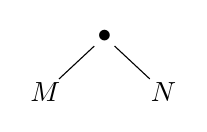
\begin{tikzpicture}[baseline=-3pt,level distance=7mm,
		every node/.style={inner sep=1pt}]
		\node {$\bullet$}
		child { node {$M$} }
		child { node {$N$} };
	\end{tikzpicture}
\]
This mapping is bijective between program terms (modulo $\alpha$-conversion) and
labeled elements of $\mathcal{C}$.

Pairs-expansions of combinators---for example the standard expansions of
$\mathrm{S}$ and $\mathrm{K}$ into $\lambda$-terms—produce larger trees but
remain within the Catalan family.  Thus the Catalan substrate is closed under
syntactic elaboration.

Operational semantics are likewise internal.  Both $\beta$-reduction and SKI
contraction replace subtrees with simpler subtrees while preserving the global
full-binary-tree form.  Each admissible reduction path therefore corresponds to
a trajectory within $\mathcal{C}$, and nondeterminism in reduction strategy
corresponds to branching structure within the Catalan tree itself.

This uniformity demonstrates that the Catalan substrate simultaneously captures:
\begin{enumerate}
	\item program syntax (binary application structure),
	\item program elaboration (via pairs-expansion or substitution), and
	\item program dynamics (via evaluation rewrites).
\end{enumerate}
Consequently, computation lives entirely within the Catalan family, justifying
its use as the structural substrate for the unified causal--computational model
developed in the main text.

\subsection{Illustrative Figures}

\begin{figure}[h]
	\centering
	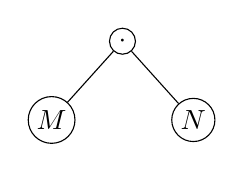
\begin{tikzpicture}[
		level distance=10mm,
		sibling distance=18mm,
		every node/.style={circle,draw,inner sep=1.5pt}
		]
		\node {$\cdot$}
			child { node {$M$} }
			child { node {$N$} };
	\end{tikzpicture}
	\caption{A binary application node representing the term $M\,N$.}
\end{figure}

\begin{figure}[h]
	\centering
	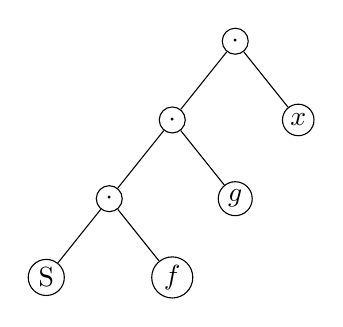
\begin{tikzpicture}[
		level distance=10mm,
		sibling distance=16mm,
		every node/.style={circle,draw,inner sep=1.5pt}
		]
		\node {$\cdot$}
			child {
				node {$\cdot$}
				child { node {$\cdot$} child { node {$\mathrm{S}$} } child { node {$f$} } }
				child { node {$g$} }
			}
			child { node {$x$} };
	\end{tikzpicture}
	\caption{Binary-tree representation of the term $\mathrm{S}\,f\,g\,x$.}
	\label{fig:Sfgx-binary-tree}
\end{figure}

\begin{figure}[h]
	\centering
	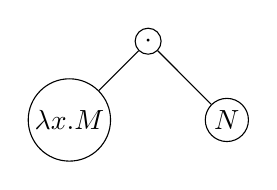
\begin{tikzpicture}[
		level distance=10mm,
		sibling distance=20mm,
		every node/.style={circle,draw,inner sep=1.5pt}
		]
		\node {$\cdot$}
			child { node {$\lambda x.M$} }
			child { node {$N$} };
	\end{tikzpicture}
	\qquad$\Longrightarrow$\qquad
	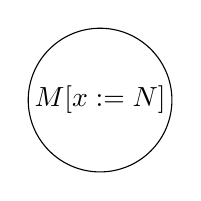
\begin{tikzpicture}[
		level distance=10mm,
		sibling distance=20mm,
		every node/.style={circle,draw,inner sep=1.5pt}
		]
		\node {$M[x:=N]$};
	\end{tikzpicture}
	\caption{$\beta$-reduction as a local rewrite inside the Catalan family.}
\end{figure}

\subsection{Pairs Expansion as Variable-Free S-Expressions}
\label{subsec:pairs-s-expressions}

A central observation motivating this work is that the pairs expansions of
combinators can be written as \emph{variable- and label-free} S-expressions,
exactly in the style of McCarthy's original Lisp notation \cite{McCarthy1960}.
In McCarthy's formulation, the core data structure is the cons-cell, written as
a parenthesized pair. Here we push this idea to an extreme: we erase all atom
labels and regard the program itself as a pure cons-tree, encoded only by
balanced parentheses.

Concretely, consider the binary application tree for the term
$\mathrm{S}\,f\,g\,x$ (as in Figure~\ref{fig:Sfgx-binary-tree}). Under the pairs
encoding used in our simulations, this same shape appears as the variable-free
S-expression
\[
	\texttt{(()(()(()())))}.
\]
This S-expression can also be understood as \emph{looking down into} the
underlying Catalan tree: the outer parentheses form the root frame, while each
\texttt{()} corresponds to a leaf. The corresponding unlabeled binary tree shape
is shown below.

\begin{center}
	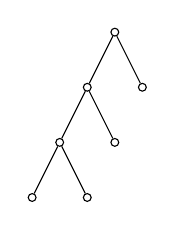
\begin{tikzpicture}[
		level 1/.style={level distance=7mm,sibling distance=7mm},
		level 2/.style={level distance=7mm,sibling distance=7mm},
		level 3/.style={level distance=7mm,sibling distance=7mm},
		every node/.style={circle,draw,inner sep=1pt,minimum size=2pt}
		]
		\node {}
			child { node {}
				child { node {}
					child { node {} }
					child { node {} }
				}
				child { node {} }
			}
			child { node {} };
	\end{tikzpicture}
\end{center}

Viewed from this perspective, the S-expression is simply the linear “parentheses
trace” of this structure: each ``('' corresponds to descending into a cons-cell,
each ``)'' corresponds to returning toward the trunk, and the empty pairs
\texttt{()} mark the terminal leaves.

More generally, the pairs bijection

\begin{small}
\begin{verbatim}
n=0, c=1:  ()
n=1, c=1:  (()())
n=2, c=2:  (()(()())) ((()())())
n=3, c=5:  (()(()(()()))) (()((()())())) ((()())(()())) ((()(()()))()) (((()())())())
\end{verbatim}
\end{small}

enumerates exactly the same Catalan shapes that appear as Dyck paths

\begin{verbatim}
n=1, c=1:  ()
n=2, c=2:  (()) ()()
n=3, c=5:  ((())) (()()) (())() ()(()) ()()()
\end{verbatim}

but seen through a different projection. The Dyck words present the
one-dimensional ``height'' profile of the walk, making the Lorentzian scaling
limit and the breadth--depth structure of the light cone transparent. The pairs
S-expressions, by contrast, foreground the \emph{binary computational
structure}: they are precisely the unlabeled S-expression trees of a Lisp-like
language, with cons as the sole constructor.
\footnote{Here “projection’’ is not a literal mapping but a change of
	coordinates on the same Catalan object. The Dyck, binary-tree, and
	S-expression representations are all related by canonical bijections; each is
	a different parametrization of the same underlying Catalan shape.  Thus
switching from Dyck words to pairs S-expressions does not change the object
itself, only the coordinate system through which it is viewed.}

In this sense, Dyck words and pairs expansions are two complementary Catalan
bijections:

\begin{itemize}
	\item Dyck words: a one-dimensional time--breadth profile well adapted to
		continuum limits and Lorentzian geometry;
	\item pairs S-expressions: a fully binary application tree well adapted to
		combinatory computation.
\end{itemize}

Both encode the same Catalan shapes; one may view them as distinct ``Lorentz
frames'' on the same underlying combinatorial substrate. The pairs expansion can
thus be regarded as an additional invariant transform: it preserves the Catalan
class while re-expressing the same light-cone structure in purely computational
coordinates.

There is also an intrinsic handedness in this picture. Dyck words of a given
semilength $n$ are not symmetric under reversal of the walk; the distribution of
shapes across the tier reflects the left-to-right order in which parentheses are
added. This asymmetry is the combinatorial trace of the fundamental handedness
of applicative collapse in the pairs expansion: application is not commutative,
and the collapse rule is oriented. The sequential construction of the
S-expression tree makes this visible as a bias in how breadth is accumulated
relative to depth.

A further simplification arises when we observe that in the S-expression view,
explicit application nodes disappear entirely. Application is seen as a
\emph{property of the parentheses themselves}: a nested pair structure is
already an applicative program. From the standpoint of Schönfinkel's combinatory
logic \cite{Schoenfinkel1924}, where even the familiar $\mathrm{S}$ and
$\mathrm{K}$ can be reduced to a single sufficiently expressive combinator, one
may heuristically say that if a lone combinator $J$ acting on parentheses is
enough, then we can omit $J$ and work directly with the bare parentheses~$()$.
The Catalan substrate then becomes a \emph{combinator-free} calculus of pure
application.

Traditional functional calculi admit multiple evaluation strategies
(normal-order, applicative-order, call-by-need, etc.). The Catalan substrate
makes explicit a natural causal preorder on redex positions (ancestor order),
constraining dependencies between contractions. Collapse is local, and
contractions supported on disjoint subtrees commute
(Lemma~\ref{lem:causal-consistency-long}). Different evaluation strategies may then
be viewed as different linearizations of the residual freedom to schedule
causally independent contractions (Appendix~\ref{appendix:computational-foundations}).

\paragraph{Historical Perspective.}

The S-expression viewpoint connects the present framework to three classical
constructions.  First, McCarthy's original Lisp treats cons-pairs as the sole
data constructor, with atoms added as a separate syntactic category
\cite{McCarthy1960}. Here we invert the hierarchy: structure is primary, and
atoms---if present at all---arise as designated structural motifs.

Second, Church encodings demonstrate that data and control structures can be
represented entirely by higher-order functions; similarly, SKI combinatory logic
eliminates variables altogether. These developments show that symbolic reference
is not primitive but can be reconstructed from purely structural or operational
primitives.

Third, Gödel numbering treats syntax as arithmetic structure. The present
approach may be viewed as a ``Catalan numbering,'' where syntactic entities are
mapped to unlabeled binary trees. The Dyck, pairs, and binary-tree bijections
then provide multiple coordinate systems for the same structural universe. In
this sense, the Catalan substrate acts simultaneously as a computational
calculus and as a structural semantics for symbolic systems.

\subsection{Symbolic Representation in a Structure-Only Substrate}
\label{subsec:symbolic-representation}

In the Catalan substrate all information is structural: the only primitive
constructor is the cons-pair, and there are no atomic labels. This raises a
fundamental question: how can a system without atoms support symbols, naming, or
reference? The answer is that symbols arise not as primitives but as
\emph{structural motifs} that function as internal or external markers depending
on context. We distinguish two forms of symbolic representation.

\subsubsection{Internal Structural Symbols}

Within a closed Catalan machine, one may bootstrap symbolic reference by
designating particular tree shapes as internal ``names.'' A higher-level
self-referential mechanism (conceptually similar to a Y-like fixed-point
operator) can maintain a dictionary of such shapes, mapping them to programs,
behaviours, or combinator expansions. In this mode, names are themselves Catalan
objects, and symbolic reference arises entirely from geometry: identifying a
symbol is equivalent to matching a structural pattern. This yields a Lisp-like
environment without atomic identifiers, where all ``atoms'' are implemented as
canonical shapes in the tree.

\subsubsection{External Structural Symbols}

When interacting with external systems, the same structural motifs can serve as
\emph{extrinsic} symbols. Distinguished shapes may encode character codes,
vector-drawing glyphs, device signals, or other forms of I/O. This does not
modify the underlying calculus: it merely overlays a conventional interpretation
on structural patterns. The Catalan substrate remains atomless internally, while
external systems treat designated shapes as meaningful codes.

\subsubsection{Unified View: Symbols as Distinguished Motifs}

Both internal and external naming mechanisms exemplify a common principle: in a
structure-only universe, symbols are not primitive entities but \emph{designated
Catalan motifs}. A symbol is simply a tree pattern endowed—internally or
externally—with stable semantic interpretation. The substrate itself does not
distinguish between data and code, or between program and identifier; all such
distinctions emerge from the placement and recognition of specific structural
forms.

\begin{definition}[Structural Symbol]

	A \emph{structural symbol} is a finite Catalan tree $S$ together with an
	interpretation map $\iota$ assigning $S$ either (i) an internal computational
	meaning within the Catalan machine, or (ii) an external semantic meaning
	communicated to an outside system. The substrate recognizes $S$ only as a
	structure; all semantics flow from~$\iota$.

\end{definition}

\begin{remark}

	Although traditional programming languages begin with atoms and build
	structure on top of them, the Catalan substrate inverts this perspective:
	structure comes first, and atoms (if needed) are reintroduced later as
	structural patterns. From this viewpoint Lisp's cons-based representation, and
	even Schönfinkel's proposal of a single universal combinator, appear naturally
	as degenerate cases of a more general structure-first semantics.

\end{remark}


\subsection{Causal Admissibility of Redex Contraction}
\label{subsec:causal-admissibility}

We now formalize the sense in which evaluation order is fixed by causality
rather than chosen by convention.

\begin{definition}[Causal Preorder on Positions]
	Let $T$ be a full binary tree in the Catalan substrate, representing a program
	term. A \emph{position} in $T$ is a node address $p$ in the usual tree sense
	(e.g.\ a finite word over $\{L,R\}$ indicating left/right choices from the
	root). We write $p \prec q$ if the node at position $p$ lies on the unique
	path from the root to the node at position $q$. The reflexive, transitive
	closure of $\prec$ defines a preorder $\preceq$ on positions, which we call
	the \emph{causal preorder}.
\end{definition}

Intuitively, $p \preceq q$ means that the subtree at $q$ is causally downstream of the subtree at $p$: any change at $p$ may propagate to $q$ but not conversely.

\begin{definition}[Redex and Causal Admissibility]
	A \emph{redex} in $T$ is a position $p$ such that the subtree rooted at $p$
	matches the left-hand side of a reduction rule (e.g.\ a $\beta$-redex or an
	SKI contraction). Let $R(T)$ be the set of all redex positions in $T$.

	A redex at position $p \in R(T)$ is \emph{causally admissible} if there is no
	other redex $q \in R(T)$ with $q \prec p$. In other words, a redex is causally
	admissible if it is minimal in $R(T)$ with respect to the strict causal order.
\end{definition}

\begin{definition}[Causally Admissible Reduction Sequence]
	A finite or infinite sequence of trees
	\[
		T_0 \to T_1 \to T_2 \to \cdots
	\]
	is \emph{causally admissible} if, for each step $T_i \to T_{i+1}$, the
	contracted redex is causally admissible in $T_i$ in the above sense. A
	\emph{causal computation} is a causally admissible sequence starting from some
	initial tree $T_0$.
\end{definition}


\begin{lemma}[Commutation of disjoint reductions]
	\label{lem:causal-consistency-long}
	Let $T$ be a Catalan tree (full binary tree) and let $p,q\in R(T)$ be two redex
	positions that are \emph{incomparable} under the causal preorder $\preceq$
	(i.e.\ neither lies on the path from the root to the other). Let $T_p$ denote
	the result of contracting the redex at $p$, and similarly $T_q$.
	Then $q$ remains a redex position in $T_p$ and $p$ remains a redex position in
	$T_q$, and contracting both redexes yields the same tree regardless of order:
	\[
		(T_p)_q \;\equiv\; (T_q)_p.
	\]
		In particular, disjoint reductions form a commuting diamond as in
		the usual commuting-diamond picture.
\end{lemma}

\begin{proof}[Proof sketch]
	Since $p$ and $q$ lie in disjoint subtrees, contracting at $p$ rewrites only
	the subtree rooted at $p$ and leaves the subtree rooted at $q$ unchanged. Thus
	the redex at $q$ is unaffected (and remains at the same position), so it may
	still be contracted in $T_p$. Symmetrically, contracting at $q$ leaves the
	subtree at $p$ unchanged. Because the two rewrite steps act on disjoint parts
	of the tree, performing both contractions yields the same result regardless of
	order.
\end{proof}


\subsection{Evaluation Strategies as Coarse-Grainings of Causal Order}
\label{subsec:evaluation-strategies}

Traditional presentations of the $\lambda$-calculus distinguish several
evaluation strategies: normal-order, applicative-order, call-by-need, and many
others. These are usually defined syntactically (e.g.\ by specifying which redex
is chosen at each step), with confluence guaranteeing that they terminate in the
same normal form when one exists. In the Catalan substrate, however, causality
constrains redex selection more tightly.

\begin{definition}[Strategy-Compatible Causal Computation]
	Let $\mathcal{S}$ be a syntactic evaluation strategy (e.g.\ normal-order or
	applicative-order) which, given a term, selects one or more redex positions
	considered ``eligible'' at each step. A causal computation
	\[
		T_0 \to T_1 \to \cdots
	\]
	is \emph{compatible} with $\mathcal{S}$ if, at each step, the contracted redex
	is both causally admissible in $T_i$ and belongs to the set of redexes
	selected by $\mathcal{S}$ for the corresponding term.
\end{definition}

\begin{proposition}[Strategies as Coarse-Grainings of Causal Structure]
	\label{prop:strategies-coarse-graining}
	Let $T_0$ be an initial term, and suppose $\mathcal{S}$ is a standard
	evaluation strategy that is normalizing on $T_0$ (e.g.\ normal-order for a
	weakly normalizing term). Then:
	\begin{enumerate}
		\item Every $\mathcal{S}$-guided reduction sequence can be refined to a
			causally admissible computation by reordering only reductions that occur
			at redexes incomparable under the causal preorder.
		\item Conversely, every causally admissible computation from $T_0$ to normal
			form projects to an $\mathcal{S}$-valid history by forgetting the precise
			interleaving of causally independent reductions.
	\end{enumerate}
	In this sense, classical evaluation strategies are coarse-grainings of the
	underlying causal order: they differ only in how they resolve the residual
	freedom to permute causally independent redex contractions.
\end{proposition}

\begin{proof}[Proof sketch]
	For (1), observe that any $\mathcal{S}$-guided sequence that temporarily
	contracts a non-minimal redex (with respect to $\preceq$) must do so in a
	context where all redexes on which it causally depends will eventually be
	contracted as well. By standard commuting-conversion arguments, we can reorder
	the sequence so that causally prior redexes are contracted first, without
	changing the final normal form. This reordering affects only redexes that lie
	in disjoint subtrees, i.e.\ are incomparable under $\preceq$.

	For (2), given a causally admissible computation, we can group together all
	contractions that $\mathcal{S}$ regards as taking place at the ``same'' redex
	position in the syntactic term, ignoring the precise ordering among
	contractions in disjoint subtrees. The resulting abstract history matches what
	$\mathcal{S}$ would produce, by confluence and the fact that $\mathcal{S}$ is
	normalizing on $T_0$. Thus $\mathcal{S}$ may be seen as a projection that
	forgets the fine-grained causal structure of independent collapses while
	preserving the global reduction behaviour.
	\end{proof}

\fi
